\chapter{Grammatical properties}\label{ch:gram}
\section{Introduction}

Having arrived at a (somewhat preliminary) definition of MVCs in Eastern Indonesia, this chapter and the subsequent ones analyse the sample according to morphosyntactic (this chapter) and semantic patterns (Chapter \ref{ch:sem}). Chapter \ref{ch:constructions} then provides a combination of grammatical and semantic traits in order to establish potentially meaningful subgroups of MVCs. As \citet{vanstaden2008serial} showed in their exploratory study on serial verbs in Eastern Indonesia, most languages in their sample did not just make use of one morphosyntactic construction type but showed variation in formal coding between different functional types. That is, out of 12 languages, only three (Buru, Kambera and Leti) had just a single morphosyntactic pattern, while all other sample languages employed at least two different construction types (Maybrat even had all four postulated construction types; see \tabref{table:VanStadenReesink2008} below). The tendency in van Staden and Reesink's data is clear: although the languages in their sample tend to favour independent serialisation (with both verbs carrying full inflection), no absolute pattern was apparent.

\begin{quote}
[...] [W]hat we can observe is a set of general tendencies in this area that needs to be further explored. One such tendency is that independent serialisation is by far the most commonly found type. Co-dependent serialisation is very common for the expression of state changes, a finding also reported for many Oceanic languages (Lynch, Ross and Crowley 2002: 47). Otherwise, predicting the construction type on the basis of the semantics is not possible. There is no good explanation for the absence of complex verbs expressing instrument and comitative, nor is there any a priori reason why co-dependent serialisation does not express comitative. \citep[48]{vanstaden2008serial}\end{quote}\nocite{LynchEtAl2002}

If there is no pattern visible in a given data set, two explanations could be tried: either there is no such pattern, regardless of how much data one may look at, or there really is a pattern, yet the resolution of the data set does not enable a clear look at it. What I want to do in this chapter is to add more data to the picture and check whether the tendencies found by van Staden and Reesink can be replicated with the EI sample. Some of the oberservations reported by van Staden and Reesink will indeed turn out to be a result of limited data. For instance, while they found that ``posture serialisation is completely absent" in East Nusantara \citep[48]{vanstaden2008serial}, the present study does have a subset of languages that make use of constructions involving a posture verb in V$_1$ (see for discussion \sectref{sec:position-action} in Chapter \ref{ch:constructions}). The main message of this chapter, however, is that pattern predictability is quite low if we just look at the morphosyntactic level (supporting the preliminary findings from \citealt{vanstaden2008serial}).

\begin{table}
\begin{tabular}{lrlrrl}
\lsptoprule
\multicolumn{1}{l}{Language}&\rotatebox{90}{Complex verbs}&\rotatebox{90}{Independent}&\rotatebox{90}{Dependent}&\rotatebox{90}{Co-dependent}&\rotatebox{90}{Totals}\tabularnewline
\midrule
\textbf{Inanwatan}& & & & &0\tabularnewline
\textbf{Mpur}& &3& &1&4\tabularnewline
\textbf{Tidore}& &5& &3&8\tabularnewline
\textbf{Hatam}& &2&3&3&8\tabularnewline
Moi&1&3& &4&8\tabularnewline
\textbf{Maybrat}&1&4&2&2&9\tabularnewline
\midrule
\textbf{Kambera}& & &1& &1\tabularnewline
Leti& &1& & &1\tabularnewline
\textbf{Buru}&4& & & &4\tabularnewline
\textbf{Tetun (Fehan)}&1&3&1& &5\tabularnewline
\textbf{Taba}& &1?&4&1&6?\tabularnewline
\midrule
Ambon Malay (Creole)&3&1& &1&5\tabularnewline
\lspbottomrule
\end{tabular}
\caption[Semantic notions expressed per construction type in each language (from van Staden & Reesink 2008: 47]{Semantic notions expressed per construction type in 12 languages from Eastern Indonesia (adapted from \citealt[47]{vanstaden2008serial}). Languages given in bold reappear in the present study. Note that Inanwatan does have \textsc{multi-verb construction}s albeit at the word level. These constructions have been excluded as proper instances of serialisation in Van Staden and Reesink, but are included in the present study.}
\label{table:VanStadenReesink2008}
\end{table}

\largerpage[-1]
One of the disadvantages of approaches like van Staden and Reesink's is that the categories are orthogonal to each other, that is, the different construction types are not based on the same invariant defining features. Rather, as already discussed in the last chapter, three major parameters have been used: independent and dependent serialisation differ in the behaviour of the morphosyntactic locus (both verbs inflected versus only one verb inflected). Co-dependent serialisation pertains to a switch in argument function, turning the direct object of V$_1$ into the subject of V$_2$. This type can occur both as independent as well as dependent serialisation. And finally, complex serialisation refers to contiguous verb sequences that share a common set of affixes (yet are different from verbal compounds by bearing independent intonational targets). Van Staden and Reesink are well aware of this categorial overlap, explicitly noting their way of dealing with it: 

\begin{quote}
[...] [A] construction can be at once be [sic] analysed as a co-dependent SVC and either an independent or dependent SVC. When both analyses were possible, we sorted this construction with the co-dependent SVCs. \citep[47]{vanstaden2008serial}
\end{quote}

The number of semantic notions coded by independent as well as dependent serialisation is therefore in fact somewhat higher in \tabref{table:VanStadenReesink2008} as co-dependency was sorted separately. In order to avoid orthogonal categories and examine the interaction between the underlying features in the EI languages, the sample is coded for single features rather than for feature bundles. The discussion in Chapter \ref{ch:theory} has evaluated a set of surface features that form the base of existing classificatory systems. Adjacency of the verbs is a key factor in Foley and Van Valin's typology into nuclear layer and core layer serialisation, and reappears in van Staden and Reesink's complex serialisation type (as a necessary prerequisite to the affix-sharing complex), as well as in Pawley's compact serialisation type (``strictly V-serialising"; \citealt[172]{pawley2008serial}). The feature \textit{locus of inflection} figures in van Staden and Reesink's distinction into independent and dependent serialisation. Argument configuration, that is, the sharing or reanalysing of arguments in a given MVC, has received most attention in cases of switch-function. Van Staden and Reesink have devoted a specific construction type to this pattern: co-dependent serialisation. And predicate-to-argument reanalysis is known to constitute a distinct construction type in Oceanic languages such as Paamese (``ambient serialisation" in Crowley's terms; \citealt{crowley2002serial}).

Therefore, for each construction in the EI sample, the features locus of inflection, argument configuration, and contiguity (of verbal constituents) were tracked as far as this was possible within the different languages. Their patterns across and within EI languages are laid out and discussed in the following sections. They are organised into three blocks: the first part of the chapter is concerned with variation in argument structure configuration. I distinguish between two broad types: Argument sharing, and no-argument sharing. Argument sharing subsumes all instances where two or more arguments are shared in the sense that there is referential identity between them. Two arguments may, for instance, be coded for different syntactic functions (object of V$_1$, subject of V$_2$), and yet refer to the same referent. The no-argument sharing type pertains to all those cases where there is no referential identity between arguments. In one subtype, however, the predicates within the MVC are intertwined by reanalysis of the first VP as subject of the second (the Paamese type mentioned above).

The second part of the chapter turns to constituent structure. Patterns in verb inflection are analysed here as variation in headedness. I will briefly introduce the concept of \textit{head} in linguistics, and discuss to what extent the phenomenon of different inflection patterns in MVCs may reflect a hierarchical organisation of MVC-internal constituents. The last section then deals with contiguity, setting the focus on the distribution of constituents within MVCs and possible limits to constituent insertion between the verbs. The chapter closes with a summary of the morphosyntactic patterns in EI MVCs and leads over to Chapter \ref{ch:sem}.

\section{Argument structure}\label{sec:argumentstructure}

Each verb in a MVC refers to its own set of referents, introducing them into the discourse space as verbal arguments, with a semantic role and a syntactic function assigned to them. Introduced arguments from different verbs in a given MVC may on all three levels -- referential status, semantic role, and syntactic function -- either combine (that is, share the same status) or refuse to do so (that is, maintain separate states). Arguments in a MVC could then in principle be analysed as being co-referential, co-thematical and co-functional, in different combinations. 

Co-functionality has long been recognised as a major feature of variation in verb serialisation, leading to classificatory systems such as van Staden \& Reesink's, where a special category is devoted to functional switch constellations (two arguments from different verbs are co-referential and co-thematical but display different functional states). 

Co-thematical semantics, that is arguments with identical semantic roles, are less well discussed. Based on a literature survey, \citet{haspelmath2016serial} puts up a classification along semantic roles rather than along syntactic functions, and calls the different types argument-role types. He basically discusses agent sharing and patient sharing, in different configurations \citep[3ff.]{haspelmath2016serial}. One type combines agent sharing with patient sharing, that is, both subjects and objects refer to the same referent and share a semantic role.

Co-referentiality, at last, is the basic underlying factor: two arguments could of course be said to be co-functional in that both are, say, subjects, but this observation is only useful if both arguments are also co-referential. Otherwise no argument-sharing would take place (function sharing between arguments of two verbal constituents as such seems rather predictable in MVCs as every VP would license its own subject). 

With these categories in mind, we can then, at least in theory, derive a set of different combinations between co-referentiality, co-thematicity, and co-func\-tion\-al\-i\-ty. \tabref{table:Combination_role-function} shows the potential combinations as well as their attestations in EI.

\begin{table}
\resizebox{\textwidth}{!}{\begin{tabular}{llccc}
  \lsptoprule
 & & {Co-referential} &{Co-thematical} & {Co-functional} \tabularnewline 
  \midrule
(i) & (Not attested?) &  x & & \tabularnewline
\tablevspace
(ii)& Switch function &  x &  x & \tabularnewline
\tablevspace
(iii) & Same subject/object &  x &  x &  x \tabularnewline
\tablevspace
(iv) & Participant introduction? &  x & &  x \tabularnewline
\tablevspace
(v) & Participant accumulation? & &  x &  x \tabularnewline
   \lspbottomrule
\end{tabular}}
\caption[Combination types of semantic role and syntactic function in shared MVC arguments]{Combination types of semantic role and syntactic function in shared MVC arguments.}
\label{table:Combination_role-function}
\end{table}

If we assume that arguments which are shared by two or more verbs necessarily refer to the same referent, we end up with the first four options from \tabref{table:Combination_role-function}: (i) the arguments are only co-referential but neither share the same semantic role nor the same syntactic function; (ii) the arguments are co-referential and in addition share the same semantic role but occur in different syntactic functions; (iii) the arguments are co-referential, co-thematical, and are expressed by the same syntactic function; or (iv) the arguments are co-referential and share the same syntactic function albeit without appearing in the same semantic role. To these four combination types, we may add a fifth one that seems to occur as a peripheral type: (v) the arguments share both semantic role and syntactic function, yet they are not (fully) co-referential.

Type (i) is not attested in the data set. Co-referentiality seems to be strongly associated either with a sharing of semantic roles, or with a sharing of syntactic function, mostly coinciding in all three categories. How could such an argument sharing look like? If one discriminates the semantic macrorole undergoer into semantic roles like patient or theme (see below for a discussion), one may regard the following example from Ewe, discussed by \citet{ameka2005multiverb} under the heading ``consecutive" MVC, as a hypothetical case of type (i):

\ea \label{ewe_3}
\langinfo{Ewe}{Niger-Congo}{\citealt[18]{ameka2005multiverb}}\\
\gll tu-i né me-mé o \\
2\textsc{sg}-grind-3\textsc{sg} \textsc{consec} 3\textsc{sg}:\textsc{neg}-fine \textsc{neg} \\
\glft `Grind it and let it not be too fine.'\\ 
\z

We can see in (\ref{ewe_3}) that both verbs refer to an object to be crushed, perhaps in a mortar. The referent is in each case assigned a different syntactic function (direct object with the first verb, subject with the second), but the semantic role is also subject to change. While the grinding requires a patient role to be filled, the stative verb clearly does not impose such a role on its subject. We may rather call it a theme. Thus, a co-referential participant is ``shared" among two verbs (and, in fact, two clauses), but is assigned different syntactic functions and different semantic roles.

Type (iii) is the most common type of argument sharing in the EI languages (as most probably also elsewhere). A same subject configuration with a subject-agent performing some action can be regarded as canonical. Example (\ref{wooi005}) from Wooi illustrates this case. The agent here is coded as subject on both verbs. The patient is the frog (referred to by \textit{ehni}) which is also the implied object of both verbs and thus also shared, as in type (iii).

\ea \label{wooi005}
\langinfo{Wooi}{Austronesian, SHWNG}{frogstory\_Kosmus}\\
\glll herava ehni hniow \\
$<$i$>$harava ehni $<$i$>$how \\
$<$3\textsc{sg}$>$lift.up one:\textsc{clf} $<$3\textsc{sg}$>$throw \\
\glft `He took one (frog and) threw (it).'\\ 
\z

Type (ii) basically covers the switch function cases: an argument receives the same semantic role twice (normally an undergoer role, most often the patient), yet the argument appears in two different syntactic functions (object of first verb, subject of second). Here is another Wooi example. The object of V$_1$, the boy and his dog, is reanalysed as subject of V$_2$, but the semantic role remains stable: in both cases, the boy and the dog are in the patient role, being subject to the action performed by the agent (the deer).

\ea 
\langinfo{Wooi}{Austronesian, SHWNG}{frogstory\_Kosmus}\\
\glll kepateta haru huntawa \\
$<$i$>$kapateta haru hu-tawa \\
$<$3\textsc{sg}$>$shake 3\textsc{du} 3\textsc{du}-fall \\
\glft `(The deer) shook them off.'\\ 
\z

Type (iv) scenarios are hard to find in the sample. They would need to have co-referential arguments with the same syntactic function, yet with different semantic roles.\footnote{Recall from Chapter \ref{ch:introduction} that Givón's classification of SVCs into functional groups included a category of case-role marking \citep{givon1991serial}. This group appears to comprise exactly these cases, and one might assume that such SVCs often feature a shift in semantic roles. Research into SVCs has found this group to be strongly prominent in African languages (Birgit Hellwig, p.c.). This tendency is only weakly mirrrored in some of the languages of Eastern Indonesia, and we shall see in Chapter \ref{ch:discussion} that, on average, other types are more predominant in the area. This points to overall differences between linguistic areas, with different ways of putting verb serialisation into practice.} One example for this type might be instrument introduction MVCs in which V$_1$ introduces an (object) referent by use of a \textsc{take} verb. V$_2$ then takes up the argument as the understood instrument with which the action is carried out. At least from a lexical-based perspective, a co-referential argument would in this scenario appear first as an object-theme, and then as an object-instrument (see e.g. \citealt[305]{Durie1997} for examples of instrument serialisation). Other potential cases of type (iv) are occasionally (though very rarely) found in constructions that are already grammaticalised to a certain extent. Here is one more example from Wooi. A directed motion verb seems to introduce an agent-theme (the goer), but is then followed by an undergoer verb, \textit{pandasia}, which has the meaning `fall into water'. This second verb certainly renders the agent-theme a patient since the action takes place accidentally and without any volitional force.

\ea 
\langinfo{Wooi}{Austronesian, SHWNG}{frogstory\_Kosmus}\\
\glll haru hunda humpandasia na \\
haru hu-ra hu-pandasia na \\
3\textsc{du} 3\textsc{du}-go 3\textsc{du}-fall.into.water \textsc{loc}.\textsc{ana} \\
\glft `The two of them fell into the water at (that place).'\\ 
\z

\largerpage[-1]
Such combinations are so uncommon in Wooi as well as across the other EI languages, however, that I suspect the \textsc{go} verb to fulfill a somewhat grammaticalised function here. The going could either be read as a sequentialising function (`then they fell into the water', as for example with \textit{lako} `go/then' in Tolaki; on Tolaki \textit{lako} see \sectref{sec:symmetrical-head}), or as some kind of aspectual or epistemological encoding which is attested for directed motion verbs in other languages (for instance, the inceptive aspect function in Moskona, cf. \citealt[297]{gravelle2010grammar}). In this scenario, the \textsc{go} verb would not license an agent-theme participant any more, and we would probably be dealing with a plain type (iii). Alternatively, the grammaticalised V$_1$ would not assign a semantic role whatsoever, but rather act like a modifier.

Of these four types, type (iii) covers the bulk of MVCs in the sample. Type (i) is not attested, type (iv) only with some dubious examples. The rest is covered by the switch function type (ii). This leaves us with type (v), co-thematical and co-functional arguments that refer to two different referents. This type has been included in the overview in \tabref{table:Combination_role-function} because there seems to be one remarkable group of MVCs that does exactly that. In participant accumulation constructions, two referents (each singular) are introduced by V$_1$ and are then combined into a new reference (dual or plural) designated by V$_2$. The type construction comes from Paamese and has been discussed by \citet[41]{crowley2002serial} under the label \textit{inclusory serialisation}. The EI sample only shows very few examples of this type, and most of them are slightly different in that other verbs are used in V$_1$, or the accumulation of participants is nested into a transport construction (e.g., I bring you we go ...). (\ref{paamese003}) has the prototypical example from Paamese:

\ea \label{paamese003}
\langinfo{Paamese}{Austronesian, Oceanic}{\citealt[41]{crowley2002serial}}\\
\glll makurik lovaha \\
ma-kuri-ko lo-va-haa \\
1\textsc{sg}:\textsc{im}.\textsc{fut}-take-2\textsc{sg} 1\textsc{du}.\textsc{in}-\textsc{im}.\textsc{fut}-go \\
\glft `I will take you away with me.'\\ 
\z


Now, co-referentiality, as we have seen, is a prerequisite for argument sharing (except for type (v) which is hardly present in the EI sample). Co-functionality can be recognised quite easily if the language in question is a subject indexer language (which applies to most of the EI languages). The third category, semantic role, is a bit trickier to pin down. Two problems are associated with it. First, it is at times difficult to determine the exact semantic role an argument represents in a given MVC. Some of these ambiguous cases are well-known from the literature (e.g. \citealt{Dowty1979, Jackendoff1990, van1997syntax}). For instance, does a \textsc{go} verb license an agent or a theme, or a combination of both, as the goer is both a willful instigator of an action, yet at the same time subject to a change in location? Or take instrument reanalysis from above: in certain constructions, a theme object of a \textsc{take} verb is reanalysed as an instrument of V$_2$ (and probably holds the instrument role also from a constructional perspective). 

A second problem pertains to the granularity of semantic analysis. Argument types can either be described as concrete verb-derived concepts (the eater and the eaten derived from the verb \textit{eat}), as weakly generalised semantic concepts (the eater $>$ agent and the eaten $>$ patient of a verb \textit{eat}, but these roles also reappear with other verbs), or as strongly generalised semantic macroroles (the eater $>$ agent $>$ actor, and the eaten $>$ patient $>$ undergoer) (see for instance \citealt{van1997syntax} on that topic). Depending on the granularity chosen, the feature \textit{co-thematical} from \tabref{table:Combination_role-function} may turn out to be assigned quite different values. Choosing a macrorole approach would require the merging of (iv) into (iii), at least for cases of instrument introduction (since both theme and instrument would be analysed as some sort of undergoer). On the other hand, choosing a finer granularity which is verb-based in its extreme (the eater and the eaten as roles only licit with an \textsc{eat} verb) would make the co-thematical criterion completely impractical to use. For all these reasons, and also because annotating weakly generalised semantic roles of the second kind was impossible to do for the whole EI sample within the scope of this book, I used a slightly different annotation scheme that draws heavily on the co-functional criterion. This scheme, I think, is able to capture the main options in argument sharing across the EI languages. \tabref{table:comparison_ref-sharing} gives the six values of the annotation scheme, with a definition, a templatic formalisation, and the equivalent sharing types discussed above. In what follows, I will use the term \textit{referentiality} as a shortform to refer to these six different types of argument interaction in MVCs.

\begin{table}
\begin{tabular}{l p{4cm} l l}
\lsptoprule
Ref value & Definition & Template & Sharing type \\ 
\midrule 
S & same subject & S$_i$ V (O) S$_i$ V (O) &  (iii), (iv) \\ 
\tablevspace
SO & same subject and object & S$_i$ V O$_k$ S$_i$ V O$_k$ & (iii) \\ 
\tablevspace
D & different subject (object-to-subject sharing) & S V O$_i$ S$_i$ V (O) & (ii) \\ 
\tablevspace
A & participant accumulation & S$_i$ V O$_k$ S$_{i+k}$ V (O) & (v) \\  
\tablevspace
E & event-to-argument & [S V (O)]$_i$ S$_i$ V & -- \\ 
\tablevspace
X & no sharing & S V (O) S V (O) & -- \\ 
\lspbottomrule 
\end{tabular} 
\caption[Comparison of referentiality and argument sharing types]{Comparison of referentiality values and argument sharing types. For sake of brevity, subject and oject have been abbreviated as ``S" and ``O" in the templates. S = Co-functional (``same subject"), SO = Transitive co-functional (``same subject and object"), D = Switch-function (``Different subject"), A = Participant accumulation, E = Event-to-argument (``Ambient"), X = no interaction, no arguments shared. The indexes \textit{i} and \textit{k} in the templates indicate co-referentiality between arguments. Note that in the event-to-argument type, the first VP is not co-referential with the subject of the second VP in a strict sense. The index here rather indicates a reanalysis from VP to (subject) argument.}
\label{table:comparison_ref-sharing}
\end{table}

\largerpage[1]
The annotation scheme distinguishes between six values: (1) same subject argument sharing (``S"); (2) same subject and same object argument sharing (``SO"); (3) different subjects argument sharing (this is the switch function type, annotated here as ``D"); (4) accumulated participants argument sharing (basically Crowley's inclusory serialisation type, here marked as ``A"); (5) event-to-argument reanalysis (in the literature often discussed as ambient serialisation, here marked as ``E"); and (6) no argument sharing whatsoever (``X"). The first two values, same subject ``S", and same subject and same object ``SO", match type (iii) from \tabref{table:Combination_role-function}. Type (ii) from \tabref{table:Combination_role-function} is captured by the third value, different subjects ``D", since these cases in the EI sample always seem to show shared semantic roles as well. The few cases from type (iv), hetero-thematical but co-functional objects in MVCs, go in the ``S" type, and have not been coded separately, because of the difficulties with assigning semantic roles, as discussed above. Type (v) is covered by the ``A" value. In addition, the two values ``E" and ``X" comprise cases with no direct argument sharing. \tabref{table:Referentiality_overview} below gives absolute numbers  for argument sharing types in the EI languages.

\begin{table}
\begin{tabular}{lrrrrrr}
  \lsptoprule
 & \multicolumn{1}{c}{S} & \multicolumn{1}{c}{SO} & \multicolumn{1}{c}{D} & \multicolumn{1}{c}{A} & \multicolumn{1}{c}{E} & \multicolumn{1}{c}{X} \tabularnewline 
  \midrule
  Austronesian & 869 &  28 & 105 &   6 &  92 &  22 \tabularnewline
  Papuan & 791 &  11 & 94 &   1 &  101 &  26 \tabularnewline
  \midrule
  Sulawesi & 222 &   0 &  7 &   1 &  32 &   6 \tabularnewline
  Nusa Tenggara & 674 &  9 &  84 &   0 &  79 &  13 \tabularnewline 
  Maluku & 193 &   7 &  24 &   2 &   33 &  14 \tabularnewline
  Western Papua & 571 &  23 & 84 &   4 &  49 &  15 \tabularnewline 
 \midrule
 Total & 1660  & 39 & 199 &  7 & 193 &  48 \tabularnewline
   \lspbottomrule
\end{tabular}
\caption[Argument structure interaction in the EI sample]{Overview of argument structure interaction in the EI languages. Note that each of the two subcalculations, i.e., into language family affiliation as well as into areal subgroups, amount to the total number of observations given in the last row.}
\label{table:Referentiality_overview}
\end{table}

What \tabref{table:Referentiality_overview} shows is that overall the same subject pattern is by far the most common argument sharing device in the EI sample, accounting in both Austronesian and Papuan languages for 1660 cases out of 2146 MVCs. The other patterns are less frequent to infrequent, as only the switch function device (``D"), and, to a lesser degree, the event-to-argument type (``E") contribute about 200 cases each. ``SO" and ``A" are almost completely absent from the sample, only appearing in very small numbers. The negative value ``X" (no argument interaction whatsoever) is also quite rare. \figref{fig:ref-family} below presents the numbers from the upper section of \tabref{table:Referentiality_overview} in percent. As can be seen, both the Austronesian and the Papuan languages are remarkably similar in the use of the different referentiality values, the distribution being almost identical. This might suggest that linguistic affiliation does not have a major influence on the choice of referentiality patterns in MVCs, at least from a global view on the EI languages.

\begin{figure}
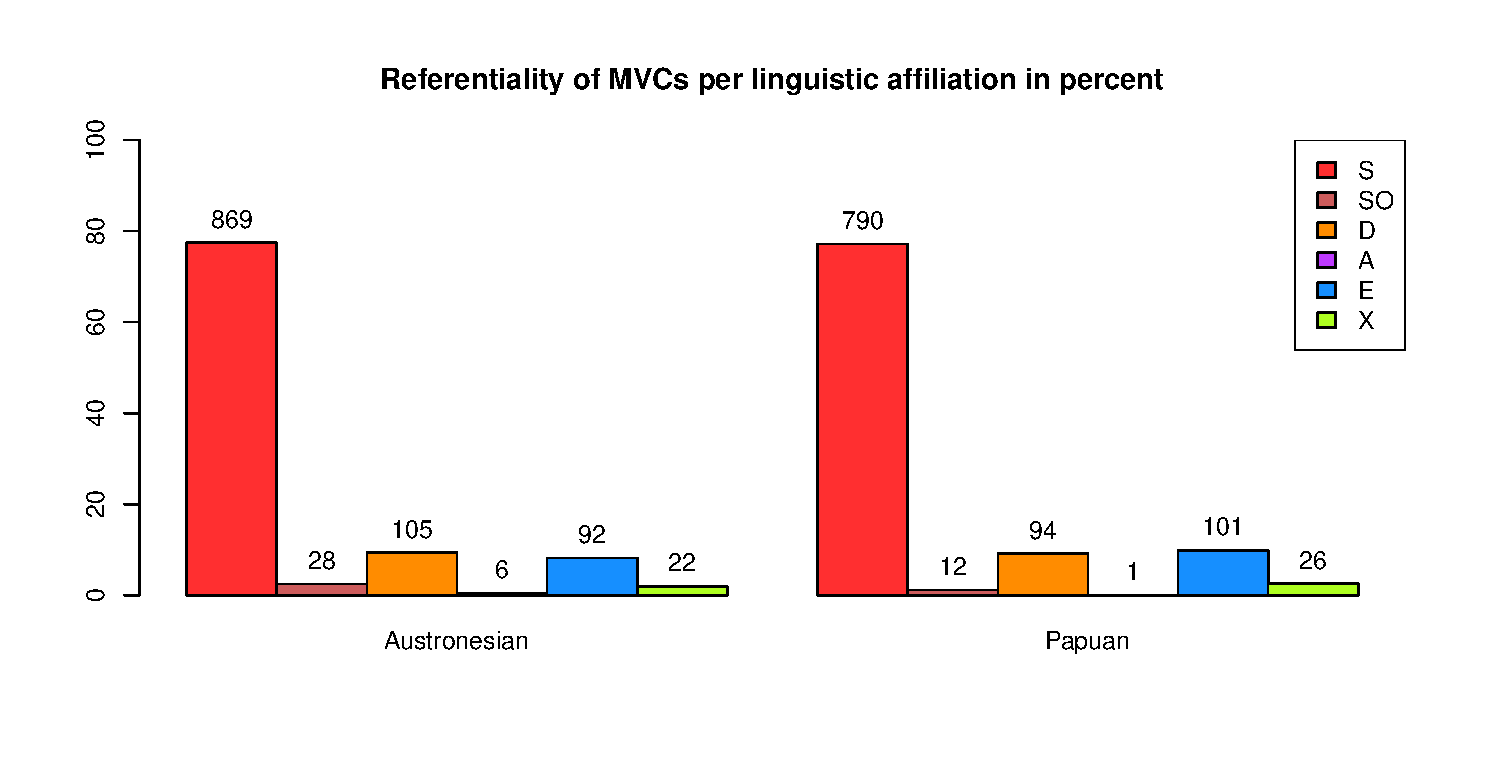
\includegraphics[width=\columnwidth]{figures/Referentiality_Family.eps}
\caption[Referentiality of MVCs per linguistic affiliation]{Referentiality of MVCs per linguistic affiliation. S = Co-functional (``same subject"), SO = Transitive co-functional (``same subject and object"), D = Switch-function (``Different subject"), A = Participant accumulation, E = Event-to-argument (``Ambient"), X = no interaction, no arguments shared. Numbers on top of the bars refer to the number of observations in the sample.}\label{fig:ref-family}
\end{figure}
\begin{figure}
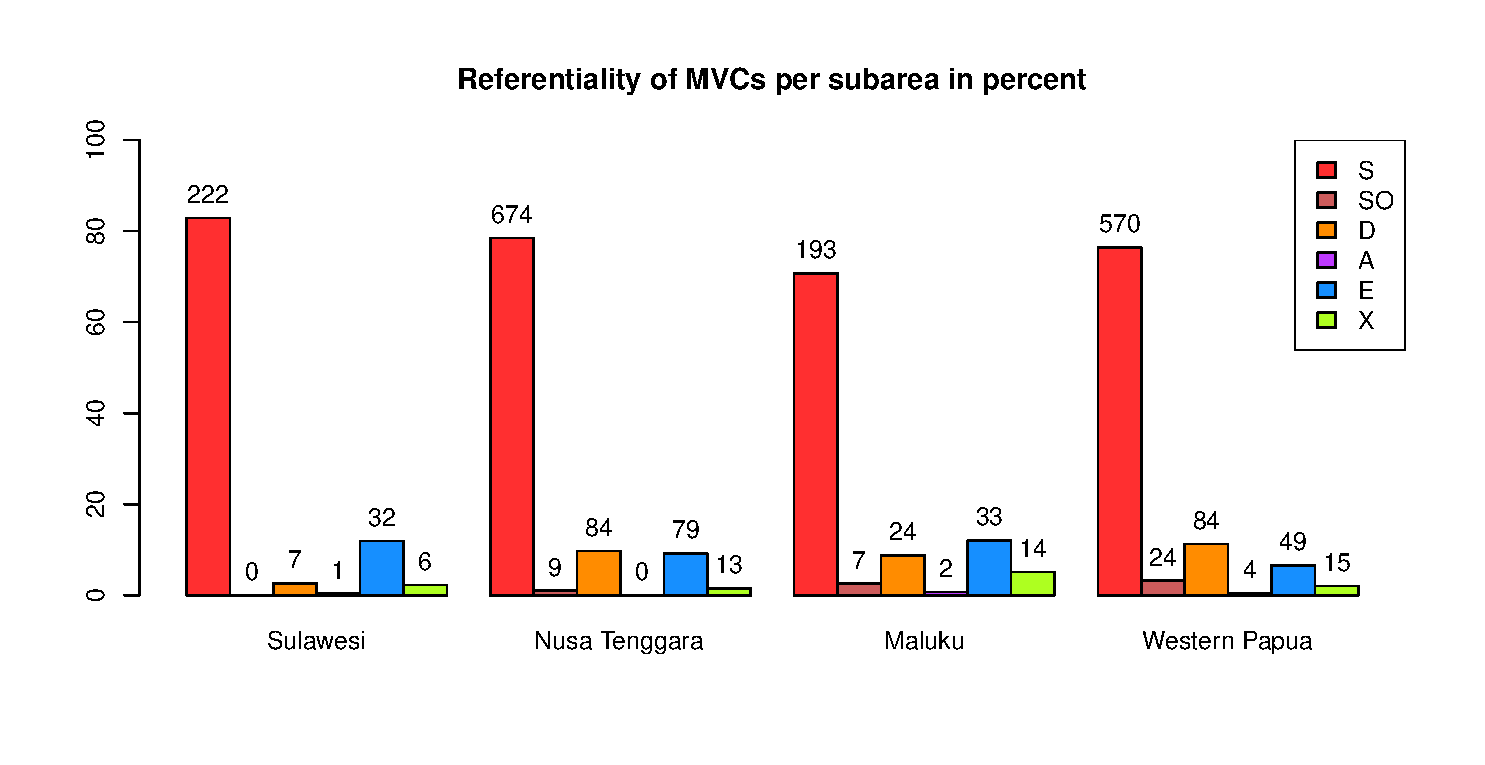
\includegraphics[width=\columnwidth]{figures/Referentiality_Group.eps}
\caption[Referentiality of MVCs per subarea]{Referentiality of MVCs per subarea. S = Co-functional (``same subject"), SO = Transitive co-functional (``same subject and object"), D = Switch-function (``Different subject"), A = Participant accumulation, E = Event-to-argument (``Ambient"), X = no interaction, no arguments shared. Numbers on top of the bars refer to the number of observations in the sample.}\label{fig:ref-group}
\end{figure}

The areal distribution patterns are quite consistent with the overall trends. \figref{fig:ref-group} again illustrates an overall similar distribution of referentiality values across subareas. Trends are hardly visible. The relation between ``D" and ``E" is subject to a certain degree of variation. While there are more ``E" than ``D" constructions in the Sulawesi and Maluku languages, Nusa Tenggara and, in particular, the Western Papua languages show the opposite pattern. Here, the ``D" pattern is more frequently encountered. Maluku also has more ``X" cases in relation to the other referentiality values than the other three groups, but this could be due to the small number of languages in this subsample (more languages might level out the overall number).

\begin{table}
\begin{tabular}{lrrrrrr}
  \lsptoprule
Language & \multicolumn{1}{c}{S} & \multicolumn{1}{c}{SO} & \multicolumn{1}{c}{D} & \multicolumn{1}{c}{A} & \multicolumn{1}{c}{E} & \multicolumn{1}{c}{X} \tabularnewline 
  \midrule
  Muna &  39 &   0 &   2 &   0 &   6 &   3 \tabularnewline 
  Pendau &  44 &   0 &   2 &   0 &   5 &   0 \tabularnewline 
  Tajio &  28 &   0 &   1 &   0 &   3 &   0 \tabularnewline 
  Tolaki &  61 &   0 &   1 &   0 &   3 &   0 \tabularnewline 
  Tukang Besi &  50 &   0 &   1 &   1 &  15 &   3 \tabularnewline 
  \midrule
  Abui & 100 &   0 &   1 &   0 &   5 &   3 \tabularnewline 
  Alorese &  36 &   0 &  11 &   0 &   0 &   0 \tabularnewline 
  Bunaq &  49 &   0 &  12 &   0 &  26 &   0 \tabularnewline 
  Kaera &  23 &   0 &   1 &   0 &   0 &   0 \tabularnewline 
  Kambera &  35 &   4 &   4 &   0 &   1 &   0 \tabularnewline 
  Klon &  94 &   0 &   3 &   0 &   2 &   1 \tabularnewline 
  Makalero &  56 &   0 &  8 &   0 &  12 &   0 \tabularnewline 
  Teiwa &  75 &   0 &   5 &   0 &   1 &   4 \tabularnewline 
  Tetun &  61 &   0 &  12 &   0 &   0 &   0 \tabularnewline 
  Waima'a & 115 &   5 &  23 &   0 &  29 &   4 \tabularnewline 
  Western Pantar &  30 &   0 &   4 &   0 &   3 &   1 \tabularnewline 
  \midrule
  Buru & 51 & 0 & 1 & 0 & 16 & 0 \tabularnewline
  Selaru &  15 &   2 &   2 &   2 &   0 &   4 \tabularnewline 
  Taba &  29 &   3 &  9 &   0 &   3 &   0 \tabularnewline 
  Tidore & 71 & 0 & 10 & 0 & 8 & 3 \tabularnewline
  Tobelo &  27 &   2 &   2 &   0 &   6 &  7 \tabularnewline 
  \midrule
  Abun &  28 &   0 &   3 &   0 &   1 &   1 \tabularnewline 
  Biak &  48 &   6 &  7 &   2 &   3 &   1 \tabularnewline 
  Dusner &  36 &   1 &  9 &   0 &   0 &   3 \tabularnewline 
  Hatam &  46 &   0 &  3 &   0 &   0 &   0 \tabularnewline 
  Inanwatan &  23 &   0 &   3 &   0 &   0 &   2 \tabularnewline 
  Maybrat &  54 &   0 &  14 &   1 &  9 &   0 \tabularnewline 
  Mor &  66 &   1 &   0 &   1 &   0 &  3 \tabularnewline 
  Moskona &  39 &   0 &  16 &   0 &  24 &   0 \tabularnewline 
  Mpur &  44 &   4 &   6 &   0 &   4 &   4 \tabularnewline 
  Sougb &  32 &   5 &   3 &   0 &   0 &   0 \tabularnewline 
  Wooi & 155 &   6 &  20 &   0 &   8 &   1 \tabularnewline 
   \lspbottomrule
\end{tabular}
\caption[Argument structure interaction per language]{Argument structure interaction per language. S = Co-functional (``same subject"), SO = Transitive co-functional (``same subject and object"), D = Switch-function (``Different subject"), A = Participant accumulation, E = Adverbial raising (``Event-to-argument"/ ``ambient"), X = no interaction, no arguments shared.}
\label{table:Referentiality_per_lang}
\end{table}

A look at the argument interaction patterns per language (\tabref{table:Referentiality_per_lang}) confirms the hypothesis that all languages make good use of the same subject pattern, making it the default argument sharing pattern in the EI area. A further interesting point is that virtually all languages (except for Mor) seem to make use of the switch function (``D") interaction pattern as well, albeit often in very low numbers. Of the other patterns, ``E" is present in all subgroups and found almost all over Sulawesi, Nusa Tenggara and Maluku. Only the Western Papua languages show less usage of this type (the bulk of examples here is from only one language, Moskona). The three other patterns are restricted to a subset of areas or even languages. ``SO" is absent from Sulawesi, and quite rare in Nusa Tenggara. Participant accumulation ``A" is virtually absent from Sulawesi and Maluku, and totally absent from Nusa Tenggara. Finally, ``X" is present in all subgroups, but only in a fraction of languages.

All in all, we may say that none of the referentiality patterns is exclusively confined to certain subareas or even to certain languages, suggesting that all patterns somehow participate in the overall dissemination of linguistic features through language contact. The fact that the ``D" pattern is in use in almost all languages would make it a particularily good candidate for an areal feature, further confirming the existence of a Sprachbund area including Sulawesi and Western Papua. This would, however, only hold true if switch function patterns could be demonstrated to be unequally distributed among serialisation languages in general. Such an assumption is difficult to validate as figures for ``D" have seldom been given. \textcite{Aikhenvald2006} and \textcite{Durie1997}, for instance, make no mention as to how many languages in fact use ``D" type SVCs in their data set. Writing on the languages of Eastern Indonesia, \citet[26]{vanstaden2008serial} state that \begin{quote}[c]o-dependent serialisation is not a very regular pattern in the East Nusantara languages. In the Austronesian languages it is only found in Taba and in Ambon Malay. It is more widely attested in the Papuan languages (Moi, Mpur, Abun, Maybrat) but it is never a frequent pattern.\end{quote}
We have just seen in \tabref{table:Referentiality_per_lang} that this assumption appears to be too pessimistic for Eastern Indonesia, and that a larger amount of data might result in the detection of more ``D" constructions. Note in particular that switch-function has now been attested in three further Austronesian languages, Buru, Kambera and Tetun Fehan, that were also part of van Staden and Reesink's sample, but for which no examples could then be found.

The following sections provide examples from the EI languages and discuss some peculiarities related to the different patterns. The sections are sorted into argument sharing and no-argument sharing patterns.

\subsection{Argument sharing}

MVCs with argument sharing amount to 1905 cases (out of 2146) in the EI sample. This means that argument sharing in general can be regarded as a core trait of MVCs, and is highly predictable. All three argument sharing types have in common some relation of shared identity between the arguments of different verbs. Co-functional MVCs, that is, the ``S" and ``SO" patterns, maintain a single syntactic function, whereas switch-function MVCs and participant accumulation MVCs do not.

\subsubsection{Co-functional MVCs}

Co-functional MVCs occur in all EI languages. As this is the default type, I will not have much to say about it. The following examples are from the four subareas, and are chosen to show different degrees of verbal subject encoding: both verbs may be closely strung together and share one set of affixes, as in example (\ref{tukangbesi003}) from Tukang Besi; both verbs may remain completely uninflected (Klon example); both verbs may be inflected for a shared subject referent, as in the Tobelo example in (\ref{tobelo001}); or only the first verb may be inflected for subject whilst the second remains bare (Hatam). Whatever the coding option, the common ground in all these constructions is that each verb refers to the same subject referent. So, for instance, in example (\ref{tukangbesi003}) the subject referent denoted by \textit{no-} is understood as being licensed by both \textit{wila} and \textit{ako}.

\ea \label{tukangbesi003}
\langinfo{Tukang Besi}{Austronesian, WMP}{\citealt[201]{donohue1999}}\\
\gll no-wila-ako-'e (na ina-no) kua daoa \\
3\textsc{rls}-go-do.for-3\textsc{obj} \textsc{nom} mother-3\textsc{poss} \textsc{all} market \\
\glft `They went for their mother to the market.'\\ 
\z

\ea 
\langinfo{Klon}{Papuan, TAP}{\citealt[137]{baird2008grammar}}\\
\gll kuur angkol a-awar qad alah mi ik \\
dog self \textsc{rdp}-return come house be.at \textsc{compl} \\
\glft `The dog itself came back and was at home.'\\ 
\z

\ea \label{tobelo001}
\langinfo{Tobelo}{Papuan, NH}{\citealt[43]{holton2003tobelo}}\\
\gll o-Morotai-iha gaanga yo-koki-boa yo-karajanga \\
\textsc{nm}-M.-\textsc{land} there 3\textsc{pl}-\textsc{dstr}-come 3\textsc{pl}-work \\
\glft `We all came to Morotai to work.'\\
\z

\ea 
\langinfo{Hatam}{Papuan, Hatam-Mansim}{\citealt[108]{reesink1999grammar}}\\
\gll yoni y-ug bong ei ig-bei big \\
they 3\textsc{pl}-go sleep \textsc{loc} house-under not \\
\glft `They don't go (to) sleep in the house (at home).'\\ 
\z

The most common sharing pattern is subject sharing, as we have seen. In case there are objects, these are often not shared (two examples for object sharing are given below; further discussion is found in \sectref{sec:handling-to-action} on handling constructions that involve both ``S" and ``SO" patterns). Object sharing is also much rarer than subject sharing as many verbs in V$_1$ position are intransitive (as is the case with the motion verbs in the examples above). This may, for instance, explain why the Sulawesi languages have no ``SO": there are hardly any combinations of transitive verbs found. When object sharing does take place in the other subareas, it always seems to involve subject sharing as well. Both verbs in such cases are of course transitive. V$_1$ more or less invariantly involves a verb of object manipulation (basically verbs of taking, and patientive manipulation verbs such as hitting, kicking, stabbing or hammering). Here are two examples of object sharing:

\ea \label{taba001}
\langinfo{Taba}{Austronesian, SHWNG}{\citealt[311]{bowden2001taba}}\\
\glll ntotas nik kos nabulang \\
n=totas nik kos n=ha-bulang \\
3\textsc{sg}=wash 1\textsc{sg}.\textsc{poss} T-shirt 3\textsc{sg}=\textsc{caus}-be.white \\
\glft `She washed my T-shirt white.'\\ 
\z

\ea \label{mpur001}
\langinfo{Mpur}{Papuan, isolate}{\citealt[98]{ode2002sketch}}\\
\gll n-soro mar ka n-da(k)-frak nton aka ut \\
3\textsc{sg}.\textsc{f}-take.off cloth that 3\textsc{sg}.\textsc{f}-take-throw child then died \\
\glft `She took off that cloth and threw the child away and it died.'\\ 
\z

Example (\ref{taba001}) from Taba is a resultative construction in which a causative verb is derived from a resultant state verb, sharing the object with the first verb, \textit{nik kos} `my T-shirt' (a more literal translation would probably be `she washed my T-shirt$_i$ causing it$_i$ to become white'). The second example in (\ref{mpur001}) is from Mpur, and shows a close combination of a \textsc{take} verb and a \textsc{throw} verb. Both verbs are transitive and license both a co-referential subject and object argument (`and took (and) threw the child away' would probably be more precise).

\subsubsection{Switch-function MVCs}

Switch-function MVCs are found in all EI languages but one (I am assuming that the missing data from Mor are most probably a chance effect). The canonical switch-function type is similar to the shared subject and object constructions (``SO") from the last section in that an event of object manipulation is viewed from two different perspectives. In the SO type, both event designators assume an agentive perspective, just as in example (\ref{mpur001}) from Mpur (actor does action A to object$_i$, actor does action B to object$_i$). The only difference in the switch-function type is that it is only the first event designator that is agent-oriented. The second verb then shifts to an undergoer perspective with the \textsc{patient} entering into subject function. Such MVCs most often express a \textsc{cause-result} or a causative relation. \citet{crowley2002serial} refers to this types as switch-subject serial verbs, and gives the following oft-cited example from Paamese:

\ea 
\langinfo{Paamese}{Austronesian, Oceanic}{\citealt[55]{crowley2002serial}}\\
\glll inau nuas vuas he:mat \\
inau ni-uasi vuasi hee-mate \\
1\textsc{sg} 1\textsc{sg}:\textsc{dist}.\textsc{fut}-hit pig 3\textsc{sg}:\textsc{dist}.\textsc{fut}-die \\
\glft `I will hit the pig to death.'\\ 
\z

The EI languages use the switch-function pattern a lot for constructions involving a causing action and a resulting action or state. In Biak, for instance, all ``D" cases are annotated as being related to some sort of causation. The following one is rather typical: the process of a glass breaking due to some involuntary action is split up into two event kernels: the agent incidentally strikes the glass (the object), and the glass (now being understood as subject of the second, intransitive verb \textit{kpéf}) shatters.

\ea 
\langinfo{Biak}{Austronesian, SHWNG}{\citealt[194]{vanheuvel2006}}\\
\glll yúf mnis gelas ine va vo, yamer kpéf i \\
y-úf mnis gelas i-ne va vo ya-mer kpéf i \\
1\textsc{sg}-take fit glass 3\textsc{sg}.\textsc{spec}-this not \textsc{sim} 1\textsc{sg}-strike.hard shatter 3\textsc{sg} \\
\glft `I did not pick up the glass rightly so that I struck and made it shatter.'\\ 
\z

Similar construals appear in many other EI languages. The agent of V$_1$ may in some cases be replaced by the instrument as such, carrying out the action, as in example (\ref{bunaq001}) from Bunaq where the machete is promoted to subject function. Here the resultant event is not expressed by a state change verb but by a stative verb, rendering it a resultative construction rather than a construal with two active verbs.

\ea \label{bunaq001}
\langinfo{Bunaq}{Papuan, TAP}{\citealt[447]{schapper2009bunaq}}\\
\gll Sore rebel, gu-bul bere pak tol haqal. \\
machete descend 3\textsc{an}-head \textsc{cntrexp}.\textsc{inan} strike broken finished \\
\glft `The machete descended (and) struck his head splitting it completely.’\\ 
\z

Example (\ref{maybrat001}) from Maybrat below illustrates another quite freqent pattern, this time with a \textsc{theme} object becoming the subject of V$_2$ in what I call \textsc{direction complex} constructions (see discussion in \sectref{sec:direction}). Literally, it would mean `Should I pour water go(es) into the thermos flask'.

\ea \label{maybrat001}
\langinfo{Maybrat}{Papuan, isolate}{\citealt[215]{dol2007grammar}}\\
\gll t-tu aya m-amo cerek a \\
1\textsc{sg}-pour water 3\textsc{u}-go thermos.flask \textsc{int} \\
\glft `Should I pour water into the thermos flask?'\\ 
\z

The switch-function concept also extends to other construction types that seem less widespread and much more specific. Example (\ref{abui003o}) from Abui illustrates a case where a quantifier verb \textit{tafuda} is interpreted to have a subject that is co-referential with the direct object of the main verb \textit{fur} (something like `he swallowed it$_i$ (it$_i$ is) all'). Note that (\ref{abui003o}) is one of very few cases in which the function switch seems to occur the other way round: it is not the object of V$_1$ that is reanalysed as subject of V$_2$, but V$_2$ has a direct object that is reanalysed as subject of V$_1$. This order is in the Abui case an effect of general rules of constituent order placing the main verb(s) last in the clause.\footnote{Unfortunately, I have hardly found any further data that would allow to expand on this issue. What seems to be going on is that there is a clash of two constraints on constituent order at work in (some) AOV languages. On the one hand, AOV languages prefer to place the main verb at the end of the construction (just as clause-chaining languages would place their final verb at the end of the chain). On the other hand, there is a general preference in MVCs to place the verbal constituents according to the sequence in which the event stages occur (principle of iconicity; see for instance \citealt{vanstaden2008serial}). As we will see in \sectref{sec:causation}, these constraints appear to interact in complex ways, and the outcome is not always predictable. In cause-result MVCs from AOV languages, for instance, temporal iconicity is sometimes preserved, and sometimes overwritten.} Cases of reversed switch-function have therefore been subsumed under the label ``D". Another reason was that the number of instances was at any rate not sufficient to argue for a referential interaction type of its own.

\ea \label{abui003o}
\langinfo{Abui}{Papuan, TAP}{\citealt[372]{kratochvil2007grammar}}\\
\gll tafuda ha-fur-i he-nil-e \\
be.all 3\textsc{pat}-swallow.\textsc{compl}-\textsc{prfv} 3\textsc{loc}-make.like.this-\textsc{ipfv} \\
\glft `He swallowed everything this way.’\\ 
\z

The Abui example illustrates MVCs in which the function switch is only implicit, and no morphology helps interpret the argument relations. In other languages, subject marking does, in principle, allow for reference tracking, but function switches between third person referents may frequently occur along the way within concatenations of verbs. This is often only indicated by the semantic context. Take the Muna example in (\ref{muna0016}) which is, with four verbs in sequence, exceptionally long for a Sulawesi MVC. Between the first verb and the second is a function switch: it is the old man that is with a stick, not the female actor from V$_1$. V$_3$ and V$_4$ then continue with the old man being the subject. Note that the indirect object suffix of the first verb refers to \textit{kamokula}, the old (man).

\ea \label{muna0016}
\langinfo{Muna}{Austronesian, WMP}{\citealt[241]{vandenberg1989}}\\
\gll no-po-ghawa-ghoo kamokula ne-katuko no-mai-ghoo no-hulo \\
3\textsc{sg}.\textsc{rls}-\textsc{recp}-meet-\textsc{io} old 3\textsc{sg}.\textsc{rls}-stick 3\textsc{sg}.\textsc{rls}-come-\textsc{io} 3\textsc{sg}.\textsc{rls}-hunt \\
\glft `She met an old man with a stick who had been hunting.'\\ 
\z

\subsubsection{Participant accumulation}

Participant accumulation, as we have seen, is rather not a typical case of argument sharing because the referent of V$_2$ is not identical with either the subject or the object of V$_1$. Rather, it is the sum of both the subject and the object referent. This entails that V$_1$ is either transitive or intransitive with a second oblique argument. In the EI languages, two ways of construing participant accumulation can be distinguished. The Paamese type from example (\ref{paamese003}) involves a \textsc{take} verb, followed by some joint action (`I take you, we go'). The EI examples differ from this pattern in that V$_1$ (or a nested MVC in the first slot of the matrix construction) denotes a motion event (like `you come (to me), we do' or `I take you here, we do'). This motion component seems to be absent in the Paamese construction. An alternative pattern is the use of a comitative function verb in V$_1$, yielding something like `I with you, we do'. The following examples from Tukang Besi and Selaru illustrate both options. Note that, strictly speaking, it is not clear in examples like (\ref{tukang003}) that the motion verb assigns a human goal argument in the first place. Alternatively, \textit{mai} might only vaguely imply a spatial origo, which, by implicature, is interpreted as being the location of the first person singular participant. In any case, participant accumulation is a rare phenomenon in EI, and clearly different from default Paamese participant accumulation.

\ea \label{tukang003}
\langinfo{Tukang Besi}{Austronesian, WMP}{\citealt[516]{donohue1999}}\\
\gll Mai to-wila-ako to-tunga-ntunga, La bela Kandokendoke. \\
come 1\textsc{pl}.\textsc{rls}-go-\textsc{appl} 1\textsc{pl}.\textsc{rls}-\textsc{red}-fish La dear Monkey \\
\glft `Let's go and do some fishing, Dear Monkey.'\\ 
\z

\ea \label{selaru001o}
\langinfo{Selaru}{Austronesian, CMP}{\citealt[120]{coward2005}}\\
\gll Y-aso sir ma r-al-a kotw ti enen desike y-or amam desike ra ma ktei. \\
3\textsc{sg}-request them \textsc{conj} 3\textsc{pl}-give-Ø food \textsc{conj} woman that 3s-with man that they.eat until done \\
\glft `He requested they give the food so that woman and that man [can] eat until done.'\\ 
\z

\subsection{No argument sharing}

MVCs without argument sharing come in two types. The first type is annotated as ``E", marking cases where the whole first VP is reanalysed as an impersonal subject referent of the second verb. The second type appears to feature two or more VPs that have no connection to each other whatsoever. This type has been labelled ``X". Both types contribute a total of 241 cases to the sample.

\subsubsection{Event-to-argument reanalysis}\label{sec:event-to-argument}

Event-to-argument reanalysis typically consists of two event kernels: an action event, and a modifying or evaluative state. The action event becomes the sole argument of the evaluative state. Event-to-argument reanalysis is an obvious feature only in those languages that use subject indexing morphology on the verb. Languages without verbal morphology do not offer direct clues for an event-to-argument relation in MVCs but certain construction types can be interpreted that way (though not uncontroversially, or so it seems). Let us begin with some examples from languages that do mark this type. Maybrat, for instance, has a smallish class of prepositional verbs. Two of these verboids, \textit{ae} `be at' and \textit{kah} `be with', occur in MVCs where their subject does not agree with the subject of the action verb. Rather, it shows the prefix for third person unmarked gender. Compare the following examples.

\ea \label{maybrat002}
\langinfo{Maybrat}{Papuan, isolate}{\citealt[80]{dol2007grammar}}\\
\ea
\gll ait y-amo m-ae amah \\
he 3\textsc{m}-go 3\textsc{u}-at house \\
\glft `He goes home.' \\ 
\ex
\gll ait y-amo y-ae amah \\ 
he 3\textsc{m}-go 3\textsc{m}-at house \\
\glft `He goes and he is at home.'\\ 
\z
\z

\newpage

\ea \label{maybrat003}
\langinfo{Maybrat}{Papuan, isolate}{\citealt[80]{dol2007grammar}}\\
\ea
\gll t-ai m-kah ara \\
1\textsc{sg}-hit 3\textsc{u}-with stick \\
\glft `I hit with a stick.' \\ 
\ex
\gll *t-ai t-kah ara \\ 
1\textsc{sg}-hit 1\textsc{sg}-with stick \\
\z
\z

The first pair in (\ref{maybrat002}) shows two ways of using the verboid \textit{ae} with a motion verb in V$_1$. It may either agree in person marking with the motion verb, yielding a motion event with successive event stages (the going, and the resultant being at the place of destination), or it may show a disagreement in person marking. In this case, as there is no other participant available that \textit{m-} could refer to, I would suggest that it represents an instance of event-to-argument reanalysis. Semantically, one could expect something like `the going of him is (directed) at the house'. The free translation given by Dol suggests that both verbs together are interpreted as denoting one single motion event (as opposed to the staged example with person marking agreement). A similar case is found with \textit{kah} in (\ref{maybrat003}) except that the event-to-argument construal is the only one permitted. Here as well, my interpretation is that it is the hitting that \textit{m-} refers to (`my hitting is with a stick').

Other contexts with event-to-argument construals pertain to adverbial \textsc{modification}. In Tukang Besi and Muna, adverbials may behave like full verbs in that they receive subject indexing morphology. Yet in many cases, no real participant is selected but the subject indexer seems to refer to the whole event which is modified. Consider the example pair from Muna below.

\ea \label{muna003}
\langinfo{Muna}{Austronesian, WMP}{\citealt[236f.]{vandenberg1989}}\\
\ea
\gll no-nea a-leni \\
3\textsc{sg}.\textsc{rls}-usual 1\textsc{sg}.\textsc{rls}-swim \\
\glft `I usually swim.' \\ 
\ex
\gll ao-nea a-leni \\ 
1\textsc{sg}.\textsc{rls}-usual 1\textsc{sg}.\textsc{rls}-swim \\
\glft `I usually swim.' \\ 
\z
\z

The two ways of construing a temporal modification in (\ref{muna003}) offer an interesting contrast in argument relation. In the first construction, ``the juxtaposed clause is semantically the subject of the first clause", according to \citet[236]{vandenberg1989}. With some such adverbial verbs, however, a second construal is possible where the subject indexer of the modifying verb agrees with the subject of the main verb. This phenomenon is called subject harmonisation by van den Berg. Some adverbial verbs always require subject harmonisation, others never do, and a third group allows optional subject harmonisation, as for instance with \textit{nea} `(be) usual'.

All the instances above quite clearly encode event-to-argument reanalysis. In languages without rigorous subject marking on the verb, however, such construals are often only indirectly inferable. In the following examples, one of the verbs seems to refer to the whole VP rather than to a concrete participant, but this is a matter of interpretation and not marked by grammatical means.

\ea \label{abui003}
\langinfo{Abui}{Papuan, TAP}{\citealt[363]{kratochvil2007grammar}}\\
\gll di=ng wahai mara \\
3\textsc{act}=see look go.up.\textsc{cont} \\
\glft `He looks up.’\\ 
\z

\ea 
\langinfo{Taba}{Austronesian, SHWNG}{\citealt[315]{bowden2001taba}}\\
\glll Lkiu kwat \\
l=kiu kwat \\
3\textsc{pl}=be.frightened be.strong(\textsc{emph}) \\
\glft `They were really frightened.' \\ 
\z

\ea \label{waimaqa007}
\langinfo{Waima'a}{Austronesian, CMP}{dom2\_kaben 219f.}\\
\gll nau hite ma'a lo, den te ma'a lo \\
know \textsc{ptl} finish \textsc{asp} hear \textsc{ptl} finish \textsc{asp} \\
\glft `(You) already know, have already heard (...)'\\ 
\z

Example (\ref{abui003}) illustrates a construal of visual perception with a path specification denoted by a directed motion verb. As a simplex predicate, \textit{mara} `go up' would license an actor, yet the MVC in (\ref{abui003}) already has an actor (which is the experiencer, introduced by the grammaticalised element \textit{=ng}). Since the context makes it clear that the experiencer is not moving upward, the best interpretation would be that the whole event of him looking is directed upwards. The next example from Taba is a similar case. \textit{Kwat} can be an independent verb in simplex predicates. Here, it seems that the event of them being frightened is taken to be the argument of \textit{kwat} (`their being frightened is strong'). The last example in (\ref{waimaqa007}) is a completive construction from Waima'a, involving the verb \textit{ma'a} that is sometimes glossed as `finish' and sometimes as `all'. As knowing and hearing are non-agentive events and no agent seems available in both MVCs, \textit{ma'a} could again be interpreted as taking the whole event as its single argument (the knowing is all/complete/finished)\footnote{It seems tempting to analyse such \textsc{finish} verbs the ``English way" as syntactically transitive verb. However, \textsc{finish} verbs in EI languages typically do not offer any clue as to their transitivity.}.

In Buru we find an intruiging example of what seems to be an event-to-ar\-gu\-ment reanalysis together with normal subject sharing. Buru offers an interesting contrast in object marking with completive MVCs. The object enclitic \textit{-h} may either attach to the matrix verb (as in example (\ref{Buru4}) below), or to the completive verb (cf. example (\ref{Buru5})). The former case seems to highlight the consumption of the item, and \textit{sepo} could be taken as showing an unmarked same subject pattern (`he ate-it (he) finished'). This case is best described as a completive construction. A more apt translation of example (\ref{Buru4}) would thus be `He ate it all'. The latter case, on the other hand, appears to reanalyse the eating process denoted by V$_1$ as its direct object (`he ate (he) finished-it' where `it' would refer back to the eating).\footnote{Alternatively, the second constructions could be analysed as a plain affix-sharing nuclear-layer construction, with \textit{-h} still referring to the object licensed by the main verb. This would, however, not directly explain the specific focus in meaning on the action.} If that were so, we would be dealing with two argument-sharing devices being active within one MVC: same subject would allow sharing the subject referent, while the object of V$_2$ would be available through event-to-argument reanalysis. Note that such an interpretation would at any rate differ from canonical cases of ``E" in that the main event is not reanalysed as the subject of an unaccusative V$_2$, but rather as the object of a transitive verb in V$_2$. 

\ea 
\langinfo{Buru}{Austronesian, CMP}{\citealt[160]{grimes1991buru}}\\
\ea \label{Buru4}
\gll da kaa-h sepo \\
3\textsc{sg} eat-\textsc{obj}.\textsc{sg} finish \\
\glft `He finished eating it. (consumption of item)' \\ 
\ex \label{Buru5}
\gll da kaa sepo-h \\ 
3\textsc{sg} eat finish-\textsc{obj}.\textsc{sg} \\
\glft `He finished eating it. (completion of action)'\\ 
\z
\z

As this brief discussion has shown, assigning the label ``E" to MVCs is a matter of interpretation in languages that do not offer direct morphosyntactic reference tracking on the verb. Therefore it should be borne in mind that the numbers for ``E" MVCs presented in this study might change under closer investigation of the underlying referential systems.

\subsubsection{Cases without argument interaction}

MVCs without any argument interaction cover a range of constructions, and can be found in most of the EI languages. Many cases involve what seems to be juxtaposed clauses without prosodic boundary cues. Prosodic units that are uttered in close succession without clear rhythmical boundary cues are known as latching in prosody research (cf. for instance \citealt{himmelmann2018}). However, the MVCs without argument interaction that I have found in the literature are more than just prosodic collocations that reflect rapid prosodic production. In most of the cases, both (or all) events encoded by the verbs are related to each other in certain recurring ways. This relation may be temporal in that both events occur simultaneously, or in explicit sequence.  Consider for instance the simultaneous construal of the verbs \textit{hupu} and \textit{tiha} from Tobelo below.

\ea 
\langinfo{Tobelo}{Papuan, NH}{\citealt[61]{holton2003tobelo}}\\
\gll to-hupu-óko ahi-kongo i-tiha \\
1-go.out-\textsc{sea} 1\textsc{poss}-tears 3-fall \\
\glft `I came out with tears falling.'\\ 
\z

Other cases rather denote conditional relations, as in example (\ref{muna004}) from Muna. Cases like this may turn out to be simple biclausal conditionals where the grammatical marker can be left out (as with \textit{ane}). Van den Berg notes that ``it is possible to add a conjunction (for example \textit{ane} `if'), which results in a conjoined construction" \citep[235]{vandenberg1989}.

\ea \label{muna004}
\langinfo{Muna}{Austronesian, WMP}{\citealt[235]{vandenberg1989}}\\
\gll nao-kesa sepaliha dua suara-no (ane) nae-lagu \\
3\textsc{sg}.\textsc{irr}-beautiful very also voice-his (if) 3\textsc{sg}.\textsc{irr}-sing \\
\glft `His voice will also be very beautiful when he sings.'\\ 
\z

\section{Constituent structure}

The next sections now turn to morphosyntactic features on the level of constituent structure. Differences in grammatical marking between the verbs of a MVC have led many to postulate differences in constructional make-up. For instance, van Staden and Reesink classify SVCs with two inflected verbs into one category, and SVCs with only one inflected verbs into another. \sectref{sec:headedness} presents an overview of inflection patterns in the EI sample, and aims at discussing the theoretical implications that these patterns may have. One way of analysis would treat inflected verbs as conceptual heads of a syntactic projection, leading in the case of van Staden \& Reesink's ``dependent type" to a potentially hypotactic construction with one verbal constituent being of higher rank than the other. An alternative approach would not grant verbal inflection the status of a head-marking device in the sense that the underlying construction would necessarily be interpreted as hypotactic. While I will argue for some structural difference between inflected and uninflected verbs, my point is that the majority of languages from the area does not explicitly use verbal morphology to systematically trace hierarchical differences in MVCs. At the same time, certain MVCs indeed carry an inflection pattern that seems induced by the construction rather than by some parameter from other linguistic planes (such as phonology).

The second parameter discussed here under the label \textit{constituent structure} is contiguity of verbal constituents. As mentioned before, contiguity (or adjacency) of verbs is another factor often recognised as being vital to SVC formation, and construction types are often said to be sensitive to strict contiguity (think again of Pawley's compact serialisation type, for instance). \sectref{sec:contiguity} will discuss contiguity in EI MVCs.

\subsection{Headedness}\label{sec:headedness}

Verbal inflection highlights the verb as being of central importance to the construction in question, or, in Bloomfield's terms, being the \textit{center} of the construction \citep{bloomfield1933language}. This central constituent is usually referred to as \textit{head}. The idea of heads in linguistics has been in use at least since Leonard Bloomfield and the American structuralist times, and, as Zwicky in his seminal paper from 1985 showed, has come with a range of different interpretations and theoretical tenets \citep{zwicky1985heads1}. 

This section proceeds as follows: I will first give a brief summary of Zwicky's account of heads, basically because he was the first to make explicit a set of competing notions that can be taken as candidates for the concept. The headedness discussion at that time was basically revolving around the \textsc{SAE} language type, with English being the example of choice. The formula was ``one clause, one (verbal) head", and few problems arose with European languages as they adhere quite well to that principle by employing verbal morphology for finiteness distinctions in a regular way. MVCs seem to be quite different. Nevertheless it is, I think, worthwhile to take the idea of heads and apply it to these structures. In order to do so, I will in \sectref{sec:unreliable} briefly review what I call unreliable inflection in EI languages. The third part of the section in \sectref{sec:wooicase} then turns to subordinate relative clauses in Wooi. Wooi relative clauses are connected to the matrix clause via two marking strategies involving differential inflection patterns. I will argue that this distinction is not a finiteness distinction of the sort required for judging head marking patterns but quite a different technique driven by constraints in argument tracking. The fourth and final part of this section returns to EI MVCs and their inflection patterns, and gives examples from different languages of the sample.

\subsubsection{Zwicky: Competing concepts}\label{sec:Zwicky}

Discussing the ambiguity of the term \textit{head}, Zwicky singled out three notions that all share the basic idea that within a given set of two components, one of them is more central and characteristic of the whole constituent. These notions are: the semantic argument (later called base in \citealt{zwicky199313}), the subcategorisand (semantic functor), and the morphosyntactic locus (later called head, as this is assumed to be the most appropriate candidate notion with regard to syntactic constituency; \citealt[3]{zwicky1985heads1}). The semantic argument relies on semantic tests: the semantic head of two elements is the one element that is of the same kind as the categorial projection of both elements.

\begin{quote}
[I]n a combination X + Y, X is the `semantic head' if, speaking very crudely, X + Y describes a kind of the thing described by X. On this basis, N is the semantic head in Det + N (\textit{those penguins} describes a kind of penguin), and VP is the semantic head in Aux + VP (\textit{will leave} describes a kind of leaving). \citep[4]{zwicky1985heads1}
\end{quote}

The subcategorisand, the second candidate for the head of a constituent, is a constituent that is restricted in its ability to occur in specific constructional slots. The most prominent instance is verbs that are subcategorised with regard to the constellation of argument positions. Zwicky gives the following examples:

\begin{quote}
The verb \textit{give} is subcategorized to occur with either NP NP or NP \textit{to} + NP as its sisters (\textit{give Kim money, give money to Kim}); \textit{donate} is subcategorized to occur only in the second of these two constructions (*\textit{donate Kim money, donate money to Kim}). \citep[5]{zwicky1985heads1}
\end{quote}

The third notion of head is the morphosyntactic locus, that is, the constituent that bears the marks of morphosynactic relation to other constituents. If, for instance, a verb (or its projection, a VP) bears marks of mood or subject agreement then it is the morphosyntactic locus of the clause. Yet, this is only one of two possible understandings of \textit{morphosynactic locus}. There is another interpretation available in which the morphosyntactic locus is on all those constituents that would \emph{potentially} bear the respective inflectional marks if the language in question has developed the appropriate morphology. Thus, not only inflecting languages would have heads but also isolating languages where the potential locus is inferable from general theory.

\begin{quote}
This is a general notion of morphosyntactic locus which is to be considered as an explication of headship in syntactic theory. The actual inflectional locus will serve as a guide to the morphosyntactic locus in specific cases, at least in languages with sufficiently rich inflectional morphology. Speaking very loosely, the morphosyntactic locus is the `potential inflectional locus', the constituent on which inflectional features will be marked if the language has the appropriate morphology. \citep[6]{zwicky1985heads1}
\end{quote}

The surface-structural interpretion of heads as morphosyntactic loci of grammatical information clearly offers the most practical starting point for typological comparison, at least in languages with overt morphology. Within the serialisation debate, claims have been made as to where the locus of inflection should go in serial verb constructions. One of the most widely read (and cited) papers on this is Durie's \textit{Grammatical structures in verb serialization} with a critical evaluation of such predictions from GB approaches (\citealt{Durie1997}; mostly focusing on Baker's indirect $\theta$-marking account). What is interesting to us at this point is that Baker indeed assumed inflected verbs in SVCs to be heads:

\begin{quote}[I]t is known that only the head of a phrase can in general carry inflectional features that originate with an element outside that phrase. Interestingly, in some serializing languages the same tense/aspect and subject agreement morphology appears on every verb in the SVC. [...]  This is exactly what the theory expects. Traditionally, tense/aspect features are copied from the lnfl node onto the head of the associated verb phrase. The fact that these features show up on both verbs in the SVC thus supports the hypothesis that both verbs are heads. \citep[523f.]{baker1989object}
 \end{quote}
 
Baker's hypothesis would require one to interpret inflection as a marker of headedness in SVCs. There are different problems associated with this. First, as we have seen in Chapter \ref{ch:area}, the languages from EI encode quite different concepts on their verbs. Would TAM-morphology on verbs in Sulawesi languages then be comparable to person indexing verb morphology in languages from Western Papua? Some TAP languages even show traces of both verbal categories, TAM and person indexing. At the same time, many of these languages have restrictions on verb inflection. This leads to a second challenge: are languages with unstable verb morphology also to be analysed as marking heads? And third, how can we deal with differences in verbal inflection across different types of constructions? Is it the construction that sets the scene, for instance, by prohibiting inflection of V$_2$, or could it be that V$_2$ has become a non-verbal item, say, a directional particle or a case-marker.

The first challenge is hard to overcome. While TAM-morphology may be seen as some kind of ``canonical inflection type" (cf. \citealt{foley2010events}), the inflectional systems found in SAE languages often also include person indexing, typically involving portmanteau morphemes bundling together different conceptual categories. In a typological study such as the present one, at least two strategies are available: first, one could only compare languages with ``identical" conceptual categories encoded on the verbs. This would leave us with TAM-languages such as Tajio and Pendau on the one hand, and person indexing languages on the other, like most of the remaining EI languages in the sample. Obvious problems would emerge, however, with languages that do both (Inanwatan would be a good example of a language combining tense marking with person indexing on its verbs). The second strategy would lump together languages with different verbal categories, on the assumption that as long as there is \emph{some} category encoded on the verbs we are dealing with a ``head".\footnote{Specific problems would arise in case different categories were marked on different verbs. There is, however, only one such case in the EI sample. In Abui, aspectual suffixes always go with the final verb, while O crossreference is applied to those verbs that are lexically specified for marking undergoer arguments. This can lead in some cases to two verbal categories, marked on different verbs. For the reasons discussed in the following section neither verbal category has been interpreted as assigning head properties in Abui. See also \sectref{sec:asymmetrical} below.} As this strategy would help avoid the above mentioned problem of deciding what to do with mixed inflectional systems, I decided to side with the lumpers rather than with the splitters, although there are obvious shortcomings with this decision. 
 
\subsubsection{Unreliable verb morphology} \label{sec:unreliable}

Let us turn to the second challenge by having another look at irregular verb-morphological systems in EI. In both the Sulawesi and Nusa Tenggara groups, a considerable portion of languages does have inflection on their verbs, but only within a subset of cases. From the introduction to the EI languages in Chapter \ref{ch:area}, we can discern three main types of unreliable inflection in EI languages: lexically determined, situationally determined or phonologically determined. To these types, we may add a fourth one, which is totally optional inflection, as found in Tidore. This section presents a short review of these types. \tabref{table:unreliable} sums up their basic properties.

\begin{table}
\begin{tabularx}{\textwidth}{l QQ}
  \lsptoprule
Type & Properties & Languages \tabularnewline 
  \midrule
Lexical & Only a subset of verbs takes inflection &  \tabularnewline
a) obligatory & Obligatory inflection of verbs in subset & Tajio, Pendau, Teiwa, Makalero \tabularnewline
b) optional & Optional inflection of verbs in subset & \textit{not attested, but see below} \tabularnewline
c) mixed & subclasses of verbs with obligatory and optional inflection & Western Pantar, Kaera, Klon, Bunaq \tabularnewline
\midrule
Situational & Properties of the NP determine whether or not person indexer appears on the verb & \tabularnewline
a) definiteness & indefinite NPs prevent inflection & Kambera \tabularnewline
b) specificity & non-specific NPs prevent inflection & Abui \tabularnewline
c) animacy & inanimate NPs prevent inflection & Western Pantar, Teiwa, Bunaq \tabularnewline
\midrule
Phonological & Phonological factors delimit inflection & Tetun Fehan, Alorese \tabularnewline
\midrule
Free & Inflection completely optional & Tidore \tabularnewline
   \lspbottomrule
\end{tabularx}
\caption[Types of unreliable inflection in EI languages]{Four types of unreliable inflection in the EI sample. Some languages are assigned two categories as they exhibit properties of both types. See \sectref{introlang} for information on the languages, and their verbal systems.}
\label{table:unreliable}
\end{table}

The first type, the lexical type, is most widespread and covers both the \textsc{sul} and the \textsc{nus} subgroups, albeit within quite different configurations. While the Sulawesi languages Tajio and Pendau have a very small class of directional verbs resisting inflection, the opposite is true for some of the Nusa Tenggara languages where the subset of verbs that do take inflection seems quite small (Makalero) or cannot be estimated from the publications (for instance, Teiwa). Whatever the exact rules of the inflectional system might be, the bottomline is that counting verbal inflection in those languages leads to differences in inflectional behaviour within certain kinds of MVCs. In Tajio, for instance, \textsc{motion-to-action} constructions with a motion verb in V$_1$ and an action verb in V$_2$  fall into two categories: head-final if the motion verb belongs to those verbs that do not inflect, or double-headed (both verbs inflect), in case \textit{jaok} `come' is in V$_1$ (being the only motion verb that does take inflection). Examples (\ref{tajio001}) and (\ref{tajio002}) below provide an illustration.

\ea \label{tajio001}
\langinfo{Tajio}{Austronesian, CMP}{\citealt[294]{mayani2013grammar}}\\
\glll tanga ndoung minyei mosisip \\
tanga mondoung minyei mo-sisip \\
middle night go.here \textsc{dyn}.\textsc{rls}-sneak \\
\glft `In the middle of the night (I) will come here to sneak around.’\\ 
\z

\ea \label{tajio002}
\langinfo{Tajio}{Austronesian, CMP}{\citealt[294]{mayani2013grammar}}\\
\glll siia najaok nongintai tetagunya \\
siia nV-jaok noN-intai te=tagu=nya \\
\textsc{3}\textsc{sg} \textsc{st}.\textsc{rls}-come \textsc{av}.\textsc{rls}-visit \textsc{nm}=friend=\textsc{3}\textsc{sg}.\textsc{poss} \\
\glft `She came to visit her friend.’\\ 
\z

The languages from the \textsc{nus} subgroup, on the other hand, do not show lack of inflection within a semantically restricted class such as motion verbs, but partition their verbal lexicon into classes that do inflect and others that do not. Let us take Western Pantar \citep{holton2010person, holton2014western} as a brief case study. Person marking in Western Pantar is based on either free pronominals or a set of bound forms. Bound person marking forms are most commonly associated with O or S arguments, but may in rare cases also mark A participants. Whether or not a given verb accepts such bound forms is lexically determined, and the verbs fall into seven different classes. One large class, consisting of both intransitive and transitive verbs, does not accept pronominal affixes at all. Another large class contains transitive verbs where the O argument is mandatorily expressed via bound forms. A small number of verbs even takes both an undergoer and an actor prefix. Example (\ref{westernpantar001}) illustrates such a case.

\ea \label{westernpantar001}
\langinfo{Western Pantar}{Papuan, TAP}{\citealt[77]{holton2014western}}\\
\gll Ke'e pi-ga-ussar. \\
fish 1\textsc{in}-3\textsc{sg}-catch \\
\glft `We are catching fish.'\\ 
\z

Exceptional A marking by bound forms is further complicated by the fact that the A and O indexers may occur in the opposite order in some examples. In addition, \citet{holton2010person} gives another five classes of verbs that optionally take bound forms. The bulk of Western Pantar motion verbs seems to go into these classes, among many other verbs. Motion verbs in Holton's class III, for instance, do not normally receive S indexers but may do so occasionally with first and second person referents \citep[109]{holton2010person}. Two examples from the EI sample illustrate this. The first example has \textit{lama} `walk'\footnote{Note that \textit{lama} is one of those items that receive differential glossing across various examples, shifting between `go' and `walk' (I changed the gloss to `go/walk' in examples (\ref{lama_1}) and (\ref{lama_2})). As Western Pantar appears to have other motion verboids meaning `go' (for instance \textit{wa}) that come to stand in path-specifying positions in \textsc{motion complex} constructions (see \sectref{sec:motioncomplex}), I have tentatively treated \textit{lama} as a manner of motion verb, rather than a pure path-denoting directional motion verb proper, although in some examples it does seem to convey path semantics as well.} uninflected, while the second one has it inflected for person. Note that both cases contain first person referents so that in principle one could also expect the opposite inflectional behaviour.

\ea \label{lama_1}
\langinfo{Western Pantar}{Papuan, TAP}{\citealt[90]{holton2014western}}\\
\gll ping dalla siga=b lama dia maum pi badde using kalung ta \\
1\textsc{sg}.\textsc{act} tomorrow there=\textsc{rel} go/walk go \textsc{level.spec.nvis} 1\textsc{pl}.\textsc{poss} fence raise here.and.there \textsc{ipfv} \\
\glft `Tomorrow we will go there and put up our fences here and there.'\\ 
\z

\ea \label{lama_2}
\langinfo{Western Pantar}{Papuan, TAP}{\citealt[88]{holton2014western}}\\
\gll pi-laku pi-lama ta \\
1\textsc{in}-two 1\textsc{in}-go/walk \textsc{ipfv} \\
\glft `Let's (just) the two of us go.'\\ 
\z

%\largerpage[-1]
The results of unreliable morphology, whether of the situational or the phonological type, are quite alike in that the inflection patterns obtained crosscut otherwise definable MVC types. This is why, in such languages, not much is gained by merely looking at the inflection patterns. The extent to which unreliable inflection obscures the sample is, however, not the same across all languages. In the Sulawesi languages, inflection on motion verbs is predictable as their behaviour is lexically conditioned. What is more, it is only a small fraction of verbs overall that do not participate in the inflection system. The picture is thus more complicated in the Nusa Tenggara languages. Here, only a small fraction of verbs (according to the inflectional remnants still active in the respective language) may display verb morphology. It is for this reason that I decided to exclude the problematic languages of this subgroup (but not of Sulawesi) from the annotation of inflection patterns in MVCs. A further complicated case is Tidore with its free choice with respect to the use of inflection on verbs. Having annotated Tidore for inflection patterns at an early stage, I later decided to keep those data included since it was not clear to me whether the appearance of verbal inflection would indeed be totally random, or whether certain inflection patterns would be favoured over others. So, when turning to a quantitative assessment of inflection patterns in \sectref{sec:headednessEI}, it must be kept in mind that the major part of the Nusa Tenggara languages have, on these grounds, been excluded from consideration.

A further complication arises with isolating languages. If a language does not have coding options on the verb in the first place, it is obvious that no insights whatsoever are gained into MVC formation by looking at its inflectional variation (as there is, of course, none). Coding Alorese, Waima'a, Buru and Abun MVCs as cases of no-head inflection would thus distort the overall picture since in these languages the question of verbal inflection characterising MVCs simply does not arise. Therefore I decided to keep these languages out of the calculation presented below.

\subsubsection{Constructional differences in head marking - the Wooi case}\label{sec:wooicase}

In this section, I would like to turn briefly to the third challenge mentioned in \sectref{sec:Zwicky} above. My main point here is that differences in inflectional behaviour do not always cue differences in headedness status, and that (lack of) inflection may be exploited quite differently in EI languages. Consider example (\ref{WBW_Agus1a}) and (\ref{WBW_Agus1b}) with relative clause constructions in Wooi.

\ea
\langinfo{Wooi}{Austronesian, SHWNG}{elicit.}\\
\ea \label{WBW_Agus1a}
\gll vaving ve rora Agus vo hanong pey no Susan \\
woman \textsc{rel} hit Agus \textsc{foc} name \textsc{ptl} \textsc{ptl} S. \\
\glft `The woman that beat Agus is named Susan.' \\ 
\newpage
\ex \label{WBW_Agus1b}
\glll vaving ve Agus riorai pay vo hanong pey no Susan \\
vaving ve Agus $<$i$>$rora=i pa-i vo hanong pey no Susan \\
woman \textsc{rel} A. $<$3\textsc{sg}$>$hit=\textsc{obj}.\textsc{sg} \textsc{h}.\textsc{prx}-\textsc{sg} \textsc{foc} name \textsc{ptl} \textsc{ptl} S. \\
\glft `The woman that Agus beat is named Susan.' \\ 
\z
\z

If a field linguist were only to elicit examples such as (\ref{WBW_Agus1a}) in order to find out about relative clauses in Wooi, he or she would get the impression that the main verb in relative clauses remains uninflected, possibly reflecting subordination. This is, however, not what is expressed by the uninflected verb here. The picture becomes clear only when the relativised argument from the main clause is not the subject of the relative clause, as in the less politically correct example in (\ref{WBW_Agus1b}). Here, we find the main verb inflected just like any ordinary main verb would be in Wooi. This difference in verb inflection remains constant across all corpus data, and is obviously driven by constraints on argument-tracking: while relativised arguments can be easily retrieved from subject function in the relative clause, tracking appears to be less straightforward with relativised arguments in postverbal object or oblique function. Therefore it seems that any shift to a non-subject function would require overt subject marking on the verb.

Does verb inflection in Wooi then always reflect issues in argument tracking? Apparently not. Take as another example motion complex MVCs in Wooi: a motion verb in V$_1$ is complemented by a directed path verb in V$_2$. This path-lending verb always remains uninflected. Here is an example from the dataset:

\ea 
\langinfo{Wooi}{Austronesian, SHWNG}{initiation\_ritual\_first\_sex}\\
\glll hembo ra o: \\
he-vo ra o: \\
3\textsc{pl}-row go \textsc{fill} \\
\glft `(Then) they row away eh -'\\ 
\z

By comparing the two construction types from Wooi I want to emphasise that verb inflection patterns may in one and the same language be exploited for quite different things. Therefore, an uncritical view on inflectional loci automatically assuming differences in constituent hierarchies would fall short of recognising precisely why these patterns emerge with certain constructions. Accordingly, in the relative clause example we would not want to claim that one type of relative clause is overtly subordinate to the matrix clause, while the other is not. The motion MVC, on the other hand, could be argued to feature different hierarchical levels (for instance, because V$_2$ is always and invariable uninflected, while other same-subject MVCs maintain subject indexing on both verbs; see also \sectref{sec:criteria_mvcs} for discussion), suggesting that the whole construction might have one clausal head (V$_1$), and another VP that is associated with it, though ranked on a lower level. But, as will become clear, verbal inflection in MVCs does not always produce such homogeneous patterns. My point in this section is that while annotating and analysing inflection on verbs in MVCs does lead to the detection of certain patterns (as we shall see below), inflectional differences in EI languages can serve different functions. The regular flagging of construction-internal hierarchies is most likely not among them, at least not in the majority of languages.

\subsubsection{Headedness variation in EI}\label{sec:headednessEI}

Headedness variation across the EI sample was annotated according to the following decision tree, leading to five different values B, 1, 2, S and N:

\begin{enumerate}
\item Is any of the verbs inflected?
\begin{enumerate}
\item None of the verbs bears inflection -- \textbf{N = None}
\item At least one verb bears inflection -- \textbf{2}
\end{enumerate}
\item Are both/all verbs inflected the same way?
\begin{enumerate}
\item Both/all verbs bear the same inflection marks -- \textbf{B = Both}
\item Verbs are inflected differently, or only one verb takes inflection -- \textbf{3}
\end{enumerate}
\item Is one set of affixes spread across more than one verb?
\begin{enumerate}
\item Two or more verbs share one set of affixes -- \textbf{S = Shared}
\item No affix sharing involved -- \textbf{4}
\end{enumerate}
\item Which verb takes inflection marks?
\begin{enumerate}
\item Only first verb is inflected -- \textbf{1 = First verb inflected}
\item Only second/final verb is inflected -- \textbf{2 = Second/final verb inflected}
\end{enumerate}
\end{enumerate}

\tabref{table:Headedness_overview} gives an overview of the distribution of these values across the EI sample. Although \citet{vanstaden2008serial} only gave numbers per semantic notion across the investigated languages (as illustrated above in \tabref{table:VanStadenReesink2008}), it seems that the trend for languages in East Nusantara is to double mark MVCs, that is, in van Staden \& Reesink's terms, use independent serialisation. This tendency is also found in the EI sample. In general, both Papuan and Austronesian languages favour symmetrical headedness patterns over non-symmetrical ones, with 412 instances of either both verbs or none of the verbs being inflected (``B" plus ``N") in the Austronesian subset, and 368 cases for the Papuan subset. The headedness type most often used in both groups is ``B", which covers van Staden \& Reesink's independent serialisation plus part of what they call co-dependent serialisation (381 instances for Austronesian languages, and 303 for Papuan languages). The second most frequent category after ``B" is ``1" in Austronesian languages, in which the first verb takes inflection but not the second, scoring higher than the no-marking pattern ``N". For the Papuan languages, both these categories are equally frequent in use. The affix-sharing type ``S" comprises van Staden and Reesink's complex serialisation as well as MVCs on word level, as for instance in Inanwatan (which had been excluded from van Staden and Reesink's data set for phonological reasons). The ``S" pattern is more frequent than the ``N" pattern in Austronesian, but not in Papuan where ``N" clearly outranks ``S".

\begin{table}
\begin{tabular}{lrrrrr}
  \lsptoprule
& \multicolumn{1}{c}{B} & \multicolumn{1}{c}{1} & \multicolumn{1}{c}{2} & \multicolumn{1}{c}{S} & \multicolumn{1}{c}{N} \tabularnewline 
  \midrule
  Austronesian & 381 & 230 &  36 &  80 & 31 \tabularnewline
  Papuan & 303 & 66 &  19 &  19 & 65 \tabularnewline
   \midrule
  Sulawesi & 117 &  69 &  29 &  27 &  26 \tabularnewline
  Nusa Tenggara & 6 & 2 &  0 &  36 & 0 \tabularnewline
  Maluku & 89 &  43 &   7 &   0 &   66 \tabularnewline 
  Western Papua & 472 & 182 &  19 &  36 &  4 \tabularnewline 
\midrule
Total & 684 & 296 & 55 & 99 & 96 \tabularnewline
\lspbottomrule
\end{tabular}
\caption[Headedness variation in the EI sample]{Overview of headedness variation in the EI languages. B = Both verbs marked, 1 = First verb marked, 2 = Second/final verb marked, S = Shared affix set, N = None of the verbs marked. Note that both subcalculations, i.e., into language family affiliation as well as into areal subgroups, each amount to the total number of observations given in the last row. Recall that all but one language from \textsc{nus} are excluded from these numbers, as well as one language from \textsc{mal} and one language from \textsc{pap}.}
\label{table:Headedness_overview}
\end{table}

Both groups, Austronesian and Papuan languages, are consistent in trending towards using ``B" above all other patterns. As \figref{fig:head-family} below illustrates, however, Austronesian languages tend to use the ``1" pattern more frequently, both in absolute numbers, and in relation to their use of ``B". Thus, in contrast to what we found with referentiality in \sectref{sec:argumentstructure}, genetic affiliation does seem to influence the likelihood of specific inflectional patterns in EI MVCs. 

The numbers for the four subareas, Sulawesi, Nusa Tenggara, Maluku and Papua, have to be read with great care. Due to the exclusion of all but one language from the \textsc{nus} group, the numbers here are identical to the distribution of inflection patterns in Kambera, the only language included in Nusa Tenggara. Another group with much noise in the results is the Maluku group. One of five languages (Buru) was excluded, and another one (Tidore) was included, but the numbers associated with it are difficult to interpret because inflection, as discussed before, seems completely optional in Tidore. The inflectional systems in Sulawesi and Western Papua were found to be stable (with the mentioned uninflected motion verbs in Pendau and Tajio). In both groups, uninflected verbs in MVCs can be interpreted as springing from properties of the respective construction, for instance, postverbs in Biak and Wooi (recall \sectref{sec:identifyingverbs} on Wooi M-verbs, \sectref{sec:cause-result} shows Biak postverbs involving causation), or preposed bare verb stems in Inanwatan (examples can be found in \sectref{sec:motioncomplex}). \figref{fig:head-group} plots the percent distribution of headedness patterns across the four subareas.

\begin{figure}
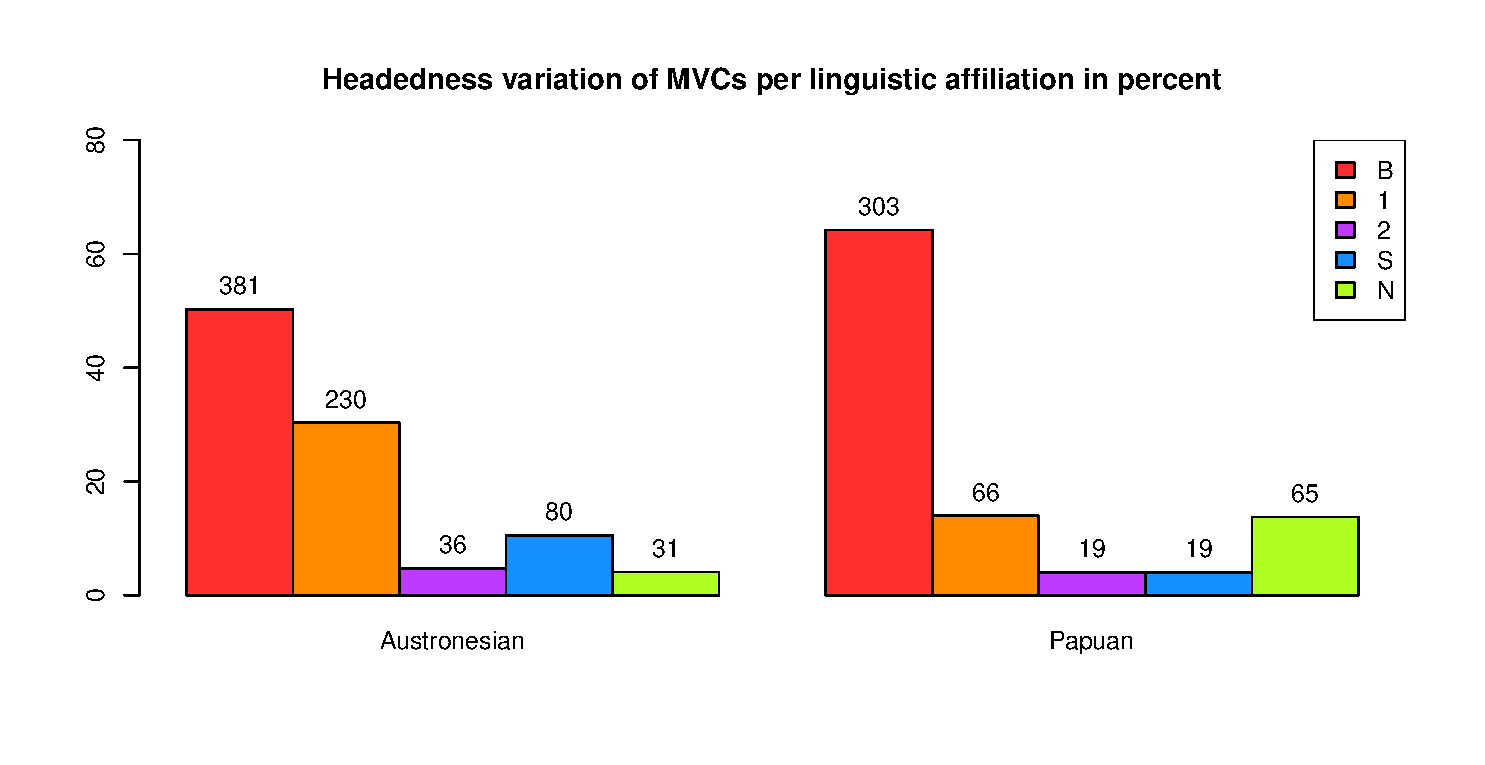
\includegraphics[width=\columnwidth]{figures/Headedness_Family.eps}
\caption[Headedness of MVCs per linguistic affiliation]{Headedness of MVCs per linguistic affiliation. B = Both verbs marked, 1 = First verb marked, 2 = Second/final verb marked, S = Shared affix set, N = None of the verbs marked. Numbers on top of the bars refer to the number of observations in the sample.}\label{fig:head-family}
\end{figure}
\begin{figure}
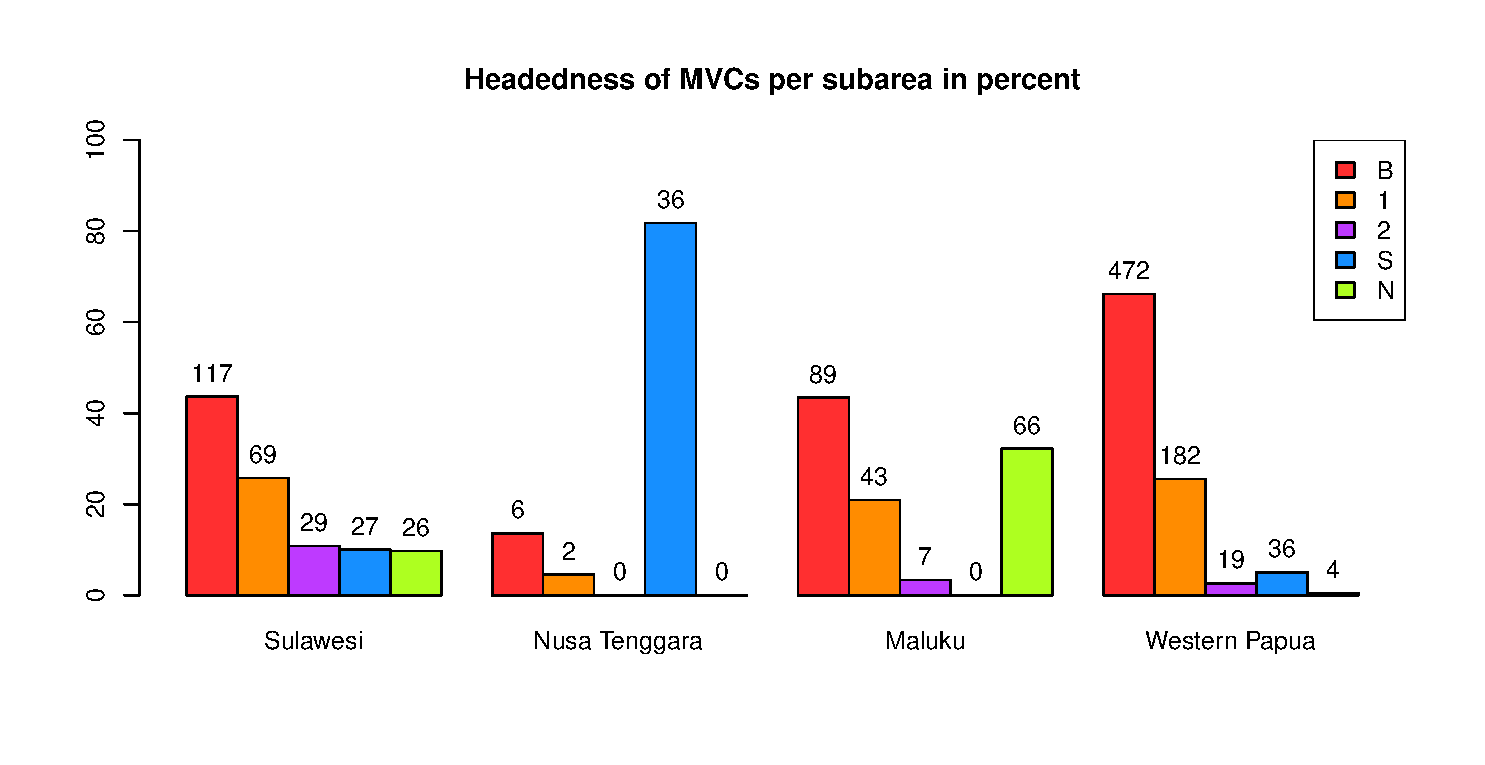
\includegraphics[width=\columnwidth]{figures/Headedness_Group.eps}
\caption[Headedness of MVCs per subarea]{Headedness of MVCs per subarea. B = Both verbs marked, 1 = First verb marked, 2 = Second/final verb marked, S = Shared affix set, N = None of the verbs marked. Numbers on top of the bars refer to the number of observations in the sample.}\label{fig:head-group}
\end{figure}

Rather surprisingly, a look at the choice of inflection patterns per language (\tabref{table:Headedness_per_lang}) clearly shows that only one language (Moskona, \textsc{pap}) sticks to a single headedness pattern for all MVCs. All other languages use more than one option (though Tobelo is another candidate for using a single pattern with only one outlier). The corpus language Wooi illustrates the full range of variation, running the whole gamut of inflectional patterns from ``B" to ``N". As with most other languages in the sample, ``B" and ``1" constitute the dominant headedness patterns in Wooi. The ``S" pattern is restricted to the cases of Wooi modifier verbs, as already introduced in \sectref{sec:identifyingverbs}). The numbers for ``2" and ``N" only reflect irregular inflectional behaviour of loan verbs from the dominant national language, Indonesian, as well as the item \textit{kay} `finish', a verboid lexeme that has undergone grammaticalisation towards a completive marker and thereby lost part of its inflectional ability. Example (\ref{wooi_andawa}) below is a combination of both an Indonesian loan verb and \textit{kay}. Such instances were counted as ``N" since no inflection could be found (nor added, for that matter).\footnote{To be precise, the verbaliser \textit{ve-} does occasionally take a prefix to mark plural subjects, but has lost the ability to inflect for singular subject referents.}

\ea \label{wooi_andawa}
\langinfo{Wooi}{Austronesian, xSHWNG}{ikan\_ANDAWA\_ANTANAY}\\
\glll mara i vo vetau kay \\
mara i vo ve-tau kay \\
\textsc{top} \textsc{3}\textsc{sg} \textsc{top} \textsc{vblz}-know complete \\
\glft `As for him, he knows all (the story).' \\ 
\z

\newpage
What is notable from \tabref{table:Headedness_per_lang} below is that there are two kinds of distributional patterns. First, there is an overall trend towards ``B" followed by ``1" (yet not in all languages). Second, there are micro trends that only take place in single languages or small clusters of neighbouring languages. For instance, all instances of ``S" marking in the Sulawesi group are due to only Tolaki and Tukang Besi, both located in the far south-east of the island. The languages from central/northern Sulawesi, Pendau and Tajio, do not seem to make use of that pattern. 

\begin{table}
\begin{tabular}{lrrrrr}
  \lsptoprule
 & \multicolumn{1}{c}{B} & \multicolumn{1}{c}{1} & \multicolumn{1}{c}{2} & \multicolumn{1}{c}{S} & \multicolumn{1}{c}{N} \tabularnewline 
  \midrule
  Muna &  46 &   0 &   4 &   0 &   0 \tabularnewline 
  Pendau &  15 &  22 &  11 &   0 &   3 \tabularnewline 
  Tajio &  18 &   4 &  10 &   0 &   0 \tabularnewline 
  Tolaki &   0 &  37 &   0 &   5 &  23 \tabularnewline 
  Tukang Besi &  38 &   6 &   4 &  22 &   0 \tabularnewline \midrule
  {\color{gray}Abui} & {\color{gray}\textit{NA}} & {\color{gray}\textit{NA}} & {\color{gray}\textit{NA}} &   {\color{gray}\textit{NA}} & {\color{gray}\textit{NA}} \tabularnewline 
  {\color{gray}Alorese} & {\color{gray}\textit{NA}} & {\color{gray}\textit{NA}} & {\color{gray}\textit{NA}} &   {\color{gray}\textit{NA}} & {\color{gray}\textit{NA}} \tabularnewline 
  {\color{gray}Bunaq} & {\color{gray}\textit{NA}} & {\color{gray}\textit{NA}} & {\color{gray}\textit{NA}} &   {\color{gray}\textit{NA}} & {\color{gray}\textit{NA}} \tabularnewline 
  {\color{gray}Kaera} & {\color{gray}\textit{NA}} & {\color{gray}\textit{NA}} & {\color{gray}\textit{NA}} &   {\color{gray}\textit{NA}} & {\color{gray}\textit{NA}} \tabularnewline
  Kambera &  6 &   2 &   0 &  36 &   0 \tabularnewline
  {\color{gray}Klon} & {\color{gray}\textit{NA}} & {\color{gray}\textit{NA}} & {\color{gray}\textit{NA}} &   {\color{gray}\textit{NA}} & {\color{gray}\textit{NA}} \tabularnewline 
  {\color{gray}Makalero} & {\color{gray}\textit{NA}} & {\color{gray}\textit{NA}} & {\color{gray}\textit{NA}} &  {\color{gray}\textit{NA}} & {\color{gray}\textit{NA}} \tabularnewline 
  {\color{gray}Teiwa} & {\color{gray}\textit{NA}} & {\color{gray}\textit{NA}} & {\color{gray}\textit{NA}} &   {\color{gray}\textit{NA}} & {\color{gray}\textit{NA}} \tabularnewline 
  {\color{gray}Tetun} & {\color{gray}\textit{NA}} & {\color{gray}\textit{NA}} & {\color{gray}\textit{NA}} &   {\color{gray}\textit{NA}} & {\color{gray}\textit{NA}} \tabularnewline 
  {\color{gray}Waimaqa} & {\color{gray}\textit{NA}} & {\color{gray}\textit{NA}} & {\color{gray}\textit{NA}} &   {\color{gray}\textit{NA}} & {\color{gray}\textit{NA}} \tabularnewline 
  {\color{gray}Western Pantar} & {\color{gray}\textit{NA}} & {\color{gray}\textit{NA}} & {\color{gray}\textit{NA}} &  {\color{gray}\textit{NA}} & {\color{gray}\textit{NA}} \tabularnewline \midrule 
  {\color{gray}Buru} & {\color{gray}\textit{NA}} & {\color{gray}\textit{NA}} & {\color{gray}\textit{NA}} & {\color{gray}\textit{NA}} & {\color{gray}\textit{NA}} \tabularnewline
  Selaru &  16 &   7 &   2 &   0 &   0 \tabularnewline 
  Taba &  24 &  18 &   1 &   0 &   1 \tabularnewline 
  Tidore & 6 & 18 & 3 & 0 & 65 \tabularnewline
  Tobelo &  64 &   0 &   1 &   0 &   0 \tabularnewline \midrule 
  {\color{gray}Abun} & {\color{gray}\textit{NA}} & {\color{gray}\textit{NA}} & {\color{gray}\textit{NA}} &   {\color{gray}\textit{NA}} & {\color{gray}\textit{NA}} \tabularnewline
  Biak &  59 &  34 &   0 &   1 &   0 \tabularnewline
  Dusner &  36 &  22 &   0 &   0 &   0 \tabularnewline
  Hatam &  47 &  29 &   0 &   0 &   0 \tabularnewline
  Inanwatan &  18 &   4 &  14 &   6 &   0 \tabularnewline
  Maybrat &  95 &   6 &   1 &   0 &   0 \tabularnewline 
  Mor &  78 &  10 &   0 &   0 &   0 \tabularnewline
  Moskona &  84 &   0 &   0 &   0 &   0 \tabularnewline
  Mpur &  74 &   7 &   1 &   1 &   0 \tabularnewline
  Sougb &  28 &   6 &   0 &   9 &   0 \tabularnewline 
  Wooi & 115 &  70 &   3 &  16 &   3 \tabularnewline
   \lspbottomrule
\end{tabular}
\caption[Headedness variation per language]{Headedness variation per language. B = Both verbs marked, 1 = First verb marked, 2 = Second/final verb marked, S = Shared affix set, N = None of the verbs marked. Languages in grey, only displaying \textsc{NA} values, have been excluded from the calculation for reasons discussed in \sectref{sec:unreliable}}
\label{table:Headedness_per_lang}
\end{table}

In the following sections, I will provide some more examples for the different inflection patterns, and try to explain the most conspicuous numbers from \tabref{table:Headedness_per_lang}. To this end, I will subsume under the label ``symmetrical-head constructions" both the ``B" and the ``N" types. ``Asymmetrical-head constructions" refer to the patterns ``1" and ``2". Finally, ``distributed-head constructions" comprise the ``S" pattern.

\subsubsection{Symmetrical-head constructions}\label{sec:symmetrical-head}

Symmetrical-head constructions mark both/all verbs in exactly the same way, that is, either they are fully inflected, or no inflection whatsoever occurs on the verbs. The latter type is of course prevalent in isolating languages of the \textsc{nus} subarea as well as in Buru, but these have been excluded for the reasons already discussed. If one just regards the languages that in principle have the grammatical means to construe asymmetrical headedness patterns, ``N" inflectional behaviour is virtually absent from all subareas, with two major exceptions. In the \textsc{mal} group, ``N" is the unmarked choice (in both senses of the term) to express MVCs in Tidore. In Sulawesi, Tolaki differs strongly from the other languages in the extent to which uninflected MVCs are in use. To illustrate this, let us have a closer look at Tolaki ``N" inflection.

\citet{mead2008verb} refer to MVCs that only have the first verb inflected as dependent serialisation, and they offer plenty of examples from Tolaki. In many of their examples, however, the first verb in sequence is not a semantically full-fledged verb that would add to the event frame of the construction, but rather a verboid with a grammatical rather than a semantic function. Therefore, when analysing such strings as a matrix construction featuring a grammaticalised verb on the one hand and a nested construction on the other, the nested construction would end up being annotated as ``N" since inflection is only attached to the matrix level verb. Here are two examples, each with a nested motion construction.

\ea \label{tolaki001}
\langinfo{Tolaki}{Austronesian, WMP}{\citealt[116]{mead2008verb}}\\
\gll lako-no-to lumaa lako um-ale-'iro banggona-no \\
go-3\textsc{sg}.\textsc{gen}-\textsc{perf} fly go $<$\textsc{m}$>$-take-3\textsc{pl}.\textsc{abs} companion-3\textsc{sg}.\textsc{gen} \\
\glft `Then he flew off and fetched his companions.' \\ 
\z

\ea \label{tolaki002}
\langinfo{Tolaki}{Austronesian, WMP}{\citealt[116]{mead2008verb}}\\
\gll a-no amba Anawaingguluri ina'u me-titiro i pu'u nohu \\
and-3\textsc{sg}.\textsc{nom} then Anawaingguluri descend $<$\textsc{m}$>$:\textsc{intr}-look-.down at base mortar \\
\glft `At that point Anawaingguluri went down and peered down at the base of the mortar.'\\ 
\z

In both (\ref{tolaki001}) and (\ref{tolaki002}) only the first verboid takes subject inflection\footnote{Note that the indexer may act as an enclitic and is then attracted to clause-initial ``single syllable relators" \citep[114]{mead2008verb}, as in (\ref{tolaki002}) where \textit{-no} is attracted to the left and the verboid \textit{amba} remains bare.}, \textit{lako} `go' (translated as `then') and \textit{amba} `then', both conveying some sequentialising function within the discourse context (next, X happened, where X is filled by a nested MVC). According to my understanding, cases like (\ref{tolaki001}) are hierarchically structured with one or more nested constructions inside (\textsc{stacked MVCs}, see also \sectref{sec:stackedmvcs}). Here, \textit{lumaa}, the second \textit{lako} and \textit{ale} together form a subordinate motion-to-action MVC which in turn has an embedded motion complex in slot 1, consisting of \textit{lumaa} and \textit{lako} (`fly go' meaning `flying off/away from situational centre'). \figref{figure:tolakiMVC} illustrates what I take to be the internal make-up of example (\ref{tolaki001}).

\begin{figure}[h]
\jtree[xunit=8em,yunit=1em]
\! = {\textit{lako lumaa lako ale}}{sequentialising}
: {\textit{lako}} {\textit{lumaa lako ale}}{motion-to-action}
: ({\textit{lumaa lako}}{motion complex}) {\textit{ale}}.
\endjtree
\caption[Internal structure of example (\ref{tolaki001}) from Tolaki]{Internal structure of example (\ref{tolaki001}) from Tolaki. Terms underneath the verbs name the respective construction.}
\label{figure:tolakiMVC}
\end{figure}

Each MVC receives its own encoding in the EI sample, and as only the topmost verb, \textit{lako}, is inflected for person, I annotated the two nested MVCs as ``N". It is this procedure that accounts for the surprising number of 23 uninflected Tolaki MVCs. Example (\ref{tolaki002}) has a similar internal structure with \textit{ina'u} `descend' and \textit{me-titiro} `look-down' forming another motion-to-action MVC.

Turning to the second type of symmetrical-head constructions, we see that in all three subareas \textsc{sul}, \textsc{mal} and \textsc{pap}, the ``B" pattern clearly dominates, with the mentioned exceptions. The following examples illustrate different inflectional categories from the subareas. In Sulawesi, mood and voice are marked on the verbs in the north, while person indexers appear on the verbs from the south-eastern languages. In Muna the mood system is integrated into the subject indexer morphology in the sense that there are two sets of indexers, one indicating realis, and another one indicating irrealis. In both Sulawesi examples below, there has to be agreement between the grammatical categories marked on the verbs: the mood values in Pendau, and the mood values as well as the person indexers in Muna. Recall that in Pendau there is a subset of motion verbs that fail to inflect, causing many motion MVCs to be either ``1" or ``2".

\ea 
\langinfo{Pendau}{Austronesian, WMP}{\citealt[355]{Quick2007}}\\
\glll a'u menyau mobanta ridagat \\
a'u \textsc{m}-pe-nyau \textsc{m}-po$_1$-banta ri=dagat \\
1\textsc{sg}.\textsc{abs} \textsc{irr}-\textsc{sf}-go.down \textsc{irr}-\textsc{sf}-fish \textsc{loc}=ocean \\
\glft `I will go down to fish in the ocean.'\\ 
\z

\ea 
\langinfo{Muna}{Austronesian, WMP}{\citealt[236]{vandenberg1989}}\\
\gll naewine da-si-kala-ha dae-kabua we tehi \\
tomorrow 1\textsc{pl}.\textsc{irr}-\textsc{si}-go-\textsc{ha} 1\textsc{pl}.\textsc{irr}-fish \textsc{loc} sea \\
\glft `Tomorrow we will go fishing together in the sea.' \\ 
\z

Selaru, Taba and Tobelo from Maluku are very similar in that they all mark subjects (in Tobelo also objects) on the verbs, and the majority of their MVCs are symmetrically inflected, with all verbs attracting inflection. Example (\ref{sel1}) from Selaru illustrates this pattern. The matrix construction is a delimitative coordination explicitly marked by use of \textit{ma}.\footnote{\textit{Ma} clearly belongs to the complex of \textsc{come} verbs that are almost ubiquitous in the EI area. Other languages like Wooi still employ cognates of this lexeme as verbs or directionals, and the verbal character is still more or less visible. Since Coward glosses \textit{ma} as a conjunction, and explicitly refers to it as a conjunctive marker, I have refrained from treating it as a verb in Selaru.} Delimitative constructions consist of both a main event and a delimiting event (x takes place \textit{until} y happens), and are mostly construed as plain biclausal constructions in EI. In this example, the first clause consists of a two-verb cause-result MVC, and both verbs, \textit{sil} `beat' and \textit{hunw} `murder', receive full person indexing inflection.

\ea \label{sel1}
\langinfo{Selaru}{Austronesian, CMP}{\citealt[125]{coward2005}}\\
\gll mw-sil-a mw-hunw-a i ma y-maty \\
2\textsc{sg}-beat-Ø 2\textsc{sg}-murder-Ø him \textsc{conj} 3\textsc{sg}-die \\
\glft `... you beat and murdered him until he died.'\\ 
\z

Symmetrical head marking is also the most common choice in the languages from Western Papua, with the exception of isolating Abun. The most consistent language in this group is Moskona with all 84 instances of MVCs in the sample being construed as ``B". Moskona is a typical West Papuan language with subject agreement prefixes on the verb and moderate verb morphology. Person marking on the verb is consistently carried out whereby third person singular subjects are zero-marked. The following two examples show position-action MVCs that have been grammaticalised to a certain extent to mark aspectual information (continuous or progressive aspect; \citealt[296]{gravelle2010grammar}). The singular example looks just like an unmarked ``N" MVC. Yet, within the Moskona subject marking paradigm, it is clear that the very same construction would receive person marking with any other person/number constellation, and so has been annotated ``B" as well.

\ea 
\langinfo{Moskona}{Papuan, EBH}{\citealt[296]{gravelle2010grammar}}\\
\gll Petrus ah omk(a) jig jog. \\
Petrus lie sleep.deep \textsc{loc} already \\
\glft `Petrus was already sleeping deeply.’ \\ 
\z

\ea 
\langinfo{Moskona}{Papuan, EBH}{\citealt[296]{gravelle2010grammar}}\\
\gll Eri i-ot i-eregejg(a) ofa. \\
they.\textsc{pl} 3\textsc{pl}-stand 3\textsc{pl}-surround s/he \\
\glft `They were (standing) around him.’\\ 
\z

\subsubsection{Asymmetrical-head constructions} \label{sec:asymmetrical}

Asymmetrical-head constructions assign verbal inflection to one of the verbs only, leaving the other(s) without prefixes or suffixes. The inflected verb may either stand in V$_1$ position (the ``1" type) or in construction-final position (``2"). If the head of a MVC is expected to go where the main verb goes in simplex clauses then one might expect that in asymmetrical-head constructions Papuan-style AOV languages would have the last verb of a MVC marked as head (see also \citealt{Durie1997} on this point). This is, however, not a consistent trend in the dataset. There are a total of nine (Papuan) languages in the sample with AOV word order of which only one language, Inanwatan from the Papua group, shows a preponderance of ``2" MVCs. All other languages are either not equipped with reliable verbal morphology (Nusa Tenggara) or do not show any inclination towards asymmetrical-head constructions at all (Tobelo from the Maluku group). As only Inanwatan behaves fully ``Papuan" in this respect, we cannot, at this point, confirm such a hypothesis. Before I take a closer look at the Inanwatan MVC system, however, I would like to make mention of one other language in the sample that seems to behave in a ``Papuan" way in terms of head-final marking.

In Abui (\textsc{nus} group), as mentioned before, there are two inflectional categories realised on the verbs. First, there is the by-now-familiar unreliable person indexing morpholgy, basically indicating undergoer arguments but at times also S. And second, there is an aspectual category with verbal suffixes denoting perfective, imperfective and durative temporal frames. It is these suffixes that seem to indicate that the last verb in a MVC could indeed be interpreted as a Papuan final verb, or at any rate as the head of the construction. When there is an aspectual suffix, it always seems to go with the last verb \citep[350]{kratochvil2007grammar}. However, as these aspectuals are not obligatory, and do not appear with every MVC, I did not count those instances as inflection. It might very well be the case that aspectual behaviour is a better indicator of headedness in Abui MVCs than unreliable person indexing.  

\largerpage[1]
Inanwatan appears to be the only language in the sample that consistently makes use of the ``2" pattern in certain MVCs. The structure is bare verb - subject indexer - second verb - tense suffix. De Vries refers to those constructions as complex phrasal verbs \citep[57]{devries2004}. The second verb slot involves most often a (directed) motion verb, but other combinations are found as well. Examples (\ref{inan1}) to (\ref{inan3}) illustrate the pattern. Recall from \sectref{sec:westpapua2} that verb inflection in Inanwatan is marked both by prefix sets for subject and objects (indicating person and number), as well as by suffixes denoting tense and gender in third person singular forms of the subject argument. Therefore \textit{noé} `go.out' in example (\ref{inan1}), for instance, clearly stands out as a preposed bare verb stem.

\ea \label{inan1}
\langinfo{Inanwatan}{Papuan, SBH}{\citealt[48f.]{devries2004}}\\
\gll mé-se-i mé-se-i mé-se-i ewáiwa, nóe-we-i-di \\
3\textsc{sbj}-walk-\textsc{pst}.\textsc{m} 3\textsc{sbj}-walk-\textsc{pst}.\textsc{m} 3\textsc{sbj}-walk-\textsc{pst}.\textsc{m} and go.out-3\textsc{sbj}-descend-\textsc{pst}.\textsc{m} \\
\glft `He went on and on and on and he arrived.' \\ 
\z

\ea \label{inan2}
\langinfo{Inanwatan}{Papuan, SBH}{\citealt[47]{devries2004}}\\
\gll gáago-wo dópis ewái ísi-we-ge-rita-re obapasa ewái \\
side-at chamber this.\textsc{f} fill-3\textsc{sbj}-do-\textsc{hab}-\textsc{pst} gunpowder this.\textsc{f} \\
\glft `At the side they used to fill the chamber with gunpowder.'\\ 
\z

\ea \label{inan3}
\langinfo{Inanwatan}{Papuan, SBH}{\citealt[44]{devries2004}}\\
\gll tíra-tira-we-i-rita-re ewáiwa íde-wó-u-rita-re \\
take-take-3\textsc{sbj}-pierce-\textsc{hab}-\textsc{pst} and \textsc{intr}-3\textsc{sbj}-fell-\textsc{hab}-\textsc{pst} \\
\glft `They pierced it repeatedly and then it would fall.'\\ 
\z

The examples show the three main functions of the Inanwatan ``2" pattern. In (\ref{inan1}) a motion verb is combined with another motion verb to form a complex motion event. The first slot may feature different motion verbs, such as \textit{mo} `come', \textit{mogo} `carry' or \textit{qai} `follow', while the second slot hosts directed motion verbs specifying the path of the motion event. The next example in (\ref{inan2}) is a loanverb carrier construction in which the loanword comes first as a bare verb stem (\textit{isi} is a loan from Indonesian \textit{(meng)isi}, `fill (into)') followed by an inflected \textsc{do} verb. This is functionally equivalent to a widespread verbaliser construction in West Papuan languages involving a form \textit{ve/be} (for instance, in Wooi and Biak). The third example in (\ref{inan3}) shows another use of the pattern. Here a \textsc{take} verb in V$_1$ is combined with some other action verb in V$_2$. \textit{Tira} may have already lost part of its lexical semantics in this construction, and could possibly express some kind of direct or total effectedness of the patient of \textit{i} `pierce'. In Tetun Fehan, for instance, the \textsc{take} -- action construction grammaticalises into a marker of successful action. In (\ref{inan3}), however, we can still recognise a typical cause-result structure `take something (and) pierce it (immediately)'. Note that the reduplication pattern suggests that both verbs indeed form a tight semantic unit: although it is the first verb \textit{tira} that is reduplicated, it seems clear from the given translation that it is an action of repeated piercing, not of repeated taking followed by a single piercing action.

\subsubsection{Distributed-head constructions}

Distributed-head constructions share a set of affixes, and both verbs seem to receive the same constituent status. Alternatively, one could analyse both verbs as forming one phrasal head instead of a lexical head. This head marking pattern is quite closely related to van Staden and Reesink's concept of complex serialisation in that both verbs form what is perceived to be an inseparable unit. Unlike Van Staden and Reesink, however, I also included cases in which both verbs appear within one phonological word (that is, having just one main accent). Distributed-head constructions are quite rare in the sample. They seem to be absent from the Moluccan languages, and appear only in a very small subset of languages in the other three subareas. In the \textsc{sul} group, the ``S" pattern is confined to south-eastern Tolaki and Tukang Besi (but not Muna). The pattern then reappears prominently in Kambera, and is used consistently in Inanwatan, Sougb, and Wooi.

Detecting distributed-head constructions is less straightforward than detecting other inflectional patterns. This is because the pattern stands out clearly only if a given language employs both prefixes and suffixes. This is the case in Tukang Besi, Kambera, and Wooi, but not in Tolaki and Sougb. My analysis of these languages should therefore be treated with some caution. Turning to the unambiguous cases first, the following examples provide illustrations of "S"-inflected MVCs in Tukang Besi and Kambera. Tukang Besi ``S" MVCs are headed by a subject indexer in the prefix slot and may have an object pronominal form at the end of the complex. Object agreement in Tukang Besi changes the argument alignment in that a full object NP must be marked with the nominative case instead of using the non-nominative core-article \textit{te}. The use of object indexers ``implies perfectivity, greater individuation of the object, and more total affectedness of the object" \citep[135]{donohue1999}. It is thus not directly connected to a certain type of MVC encoding but is instead sensitive to expressing grammatical or discourse notions.

\ea \label{tukang001}
\langinfo{Tukang Besi}{Austronesian, WMP}{\citealt[182]{donohue1999}}\\
\ea
\gll no-helo'a te roukau ako te ana-no \\
3\textsc{rls}-cook \textsc{core} vegetables do.for \textsc{core} child-3\textsc{poss} \\
\glft `She cooked the vegetables for her children.' \\ 
\ex \label{tukang001b}
\gll no-helo'a-ako te ana-no te roukau \\ 
3\textsc{rls}-cook-do.for \textsc{core} child-3\textsc{poss} \textsc{core} vegetables \\
\glft `She cooked the vegetables for her children.' \\ 
\z
\z

\ea \label{tukang002}
\langinfo{Tukang Besi}{Austronesian, WMP}{\citealt[183]{donohue1999}}\\
\gll no-tutu-molobu-'e na kabali te La Mbagi \\
3\textsc{rls}-pound-straight-3\textsc{obj} \textsc{nom} machete \textsc{core} La Mbagi \\
\glft `La Mbagi beat the machete blade straight.' \\ 
\z

The first example pair (\ref{tukang001}) shows a non-contiguous construal with the two verbs, \textit{helo'a} and \textit{ako}, being placed in separate VPs, and a contiguous construal with both verbs appearing within what seems to be one phonological unit. As no clear semantic difference is given, it seems that both constructions convey more or less the same meaning (this seems rather exceptional among EI MVCs). The undergoer arguments in both constructions are marked with the \textsc{core} marker \textit{te}. \footnote{Note that each of the verbs assigns a \textsc{core} case role to a referent. As these referents, the O and the G argument, are not co-referential one might wonder if this does not instead suggest a biclausal construal. Example (\ref{tukang001b}) therefore seems to combine contradictory signals: while the full phonological integration of both verbs appears to mirror a tight syntactic unit, the case assignment to the arguments suggests two independent argument sets, and thus a biclausal construal rather than a monoclausal one.} The last example in (\ref{tukang002}) illustrates another way of construing a clear ``S" inflectional pattern in Tukang Besi. This type is found with unaccusative verbs in V$_2$ position, and involves a switch-function interpretation (the O argument of V$_1$ becomes the S argument of V$_2$). Note that the use of the object suffix results in a switch in case-marking: the A argument is now marked with the \textsc{core} marker \textit{te} and the O argument receives nominative marking.

The Kambera ``S" pattern is quite similar to the Tukang Besi pattern. The (two) verbs are placed in clause-initial position framed by one or more person indexer(s) in prefix and/or suffix position, and aspectual suffixes. The following examples illustrate typical cases. In (\ref{kambera001}) two motion verbs are combined to form a motion complex. In this construction, the first verb seems to have lost its andative path semantics and V$_2$ \textit{mai} contributes a path specification instead. This kind of motion combination is also found in other languages of the area (for instance, in Wooi). The ``S" inflectional pattern is clearly marked off with the nominative marker in front and the imperfective clitic \textit{-pa}. Prefix indexers can, however, also be absent, as in the following example (\ref{kambera002}). Here, the first verb of the MVC, \textit{taka} `arrive', does not literally evoke a spatial dislocation of the subject but rather performs a sequentialising function. As the nominative marker is not repeated, there is no prefix indicating the ``S" pattern. Yet my interpretation here is that as long as a prefix is licit, cases like this one should also be included in the ``S" group. In other words, if there is a slot for a given affix, and there are contexts in which the use of the affix is prevented, the whole construction nonetheless conforms to the ``S" pattern.

\ea \label{kambera001}
\langinfo{Kambera}{Austronesian, CMP}{\citealt[339]{klamer1998grammar}}\\
\gll na-laku mái-pa pa-hili karai-ka \\
3\textsc{sg}.\textsc{nom}-go come-\textsc{ipfv} \textsc{ctr}-again ask-1\textsc{sg}.\textsc{acc} \\
\glft `He came yet again to ask me again.'\\ 
\z

\ea \label{kambera002}
\langinfo{Kambera}{Austronesian, CMP}{\citealt[357]{klamer1998grammar}}\\
\gll ba reu-reu padua-na-ka dá, tàka njàrung-na-nya-ka dumu \\
\textsc{conj} \textsc{rdp}-talk in\_the\_middle-3\textsc{sg}.\textsc{gen}-\textsc{perf} inside arrive punch-3\textsc{sg}.\textsc{gen}-3\textsc{sg}.\textsc{dat}-\textsc{perf} \textsc{emph}.2\textsc{sg} \\
\glft `(And) he (=J) was inside in the middle of talking, then he (=older brother) punched him (=J) ...'\\ 
\z

\subsection{Contiguity}\label{sec:contiguity}

Contiguity refers to the distribution of verbal constituents within a given MVC, and is applied here as a measure of distance between the verbs. Contiguous verbs in a MVC are directly adjacent to each other, only allowing for verbal morphology to intervene within their sequence. If both verbs form part of one phonological word, as for instance in Inanwatan, the MVC is coded as ``W". The most common case, however, is the ``C" pattern (contiguous yet being part of different phonological words). As \tabref{table:Contiguity_overview} shows, adjacent verbs that are phonologically independent form the most common contiguity pattern found in the EI languages, with a total of 1584 cases. Both macro affiliations, Austronesian and Papuan, overall favour the ``C" pattern over all other contiguity configurations (see also \figref{fig:adj-family} below). The other option for contiguous MVCs, the within-word pattern ``W", is only found in a few languages, mostly in the Papua group. With most languages, the ``W" pattern seems to only show up accidentally or in specific low-frequency constructions. So, for instance in Wooi, there is only erratic or obsolete use of within-word MVCs (for examples and discussion, see next section).

\begin{table}
\begin{tabular}{lrrrrrr}
  \lsptoprule
 & \multicolumn{1}{c}{W} & \multicolumn{1}{c}{C} & \multicolumn{1}{c}{1} & \multicolumn{1}{c}{2} & \multicolumn{1}{c}{3} & \multicolumn{1}{c}{4} \tabularnewline 
  \midrule
   Austronesian &   11 & 873 & 205 &  25 &  7 & 1 \tabularnewline 
   Papuan &  34 & 711 & 248 &  29 & 2 & 0 \tabularnewline 
   \midrule
   Sulawesi &   0 & 218 &  45 &   4 &   0 &   1 \tabularnewline
   Nusa Tenggara &   0 & 670 & 156 &  26 &   7 &   0 \tabularnewline
   Maluku &   8 &  203 &  56 &  6 &   0 &   0 \tabularnewline 
   Western Papua &  37 & 493 & 196 &  18 &   2 &   0 \tabularnewline 
   \midrule
   Total & 45 & 1584 & 453 & 54 & 9 & 1 \tabularnewline
\lspbottomrule
\end{tabular}
\caption[Contiguity variation in the EI sample]{Overview of contiguity variation in the EI languages. W = Within word, C = Contiguous verbs 1 = One non-verbal constituent intervening, 2 = Two non-verbal constituents intervening, 3 = Three non-verbal constituents intervening, 4 = Four non-verbal constituents intervening. Note that both subcalculations, i.e., into language family affiliation as well as into areal subgroups, amount to the total number of observations given in the last row.}
\label{table:Contiguity_overview}
\end{table}

When morphemic material intervenes between the verbal constituents, the first question is how to quantify the intervening elements. One could in principle either count morphemes, words, or constituents. I decided to adopt the last option as this would avoid biased counts of single constituents consisting of many morphemes or words. As displayed by the numbers, the EI languages frequently allowed one non-verbal constituent to appear between the verbs. Cases with more than one constituent were only rarely found, the most extreme being MVCs which seem to have their verbs separated by four constituents. Intervening constituents were in general more common in the Maluku and Papua group than in the other two groups: The ``1" pattern comprised about 30\% of the cases in  \textsc{mal} and \textsc{pap}, as opposed to just slightly below 20\% in \textsc{sul} and \textsc{nus}. \figref{fig:adj-group} shows the plots for degree of contiguity by subarea. No major deviation from the general pattern is to be seen, which again suggests that neither genetic affiliation nor subarea have any bearing on preferences in verb contiguity.

\begin{figure}
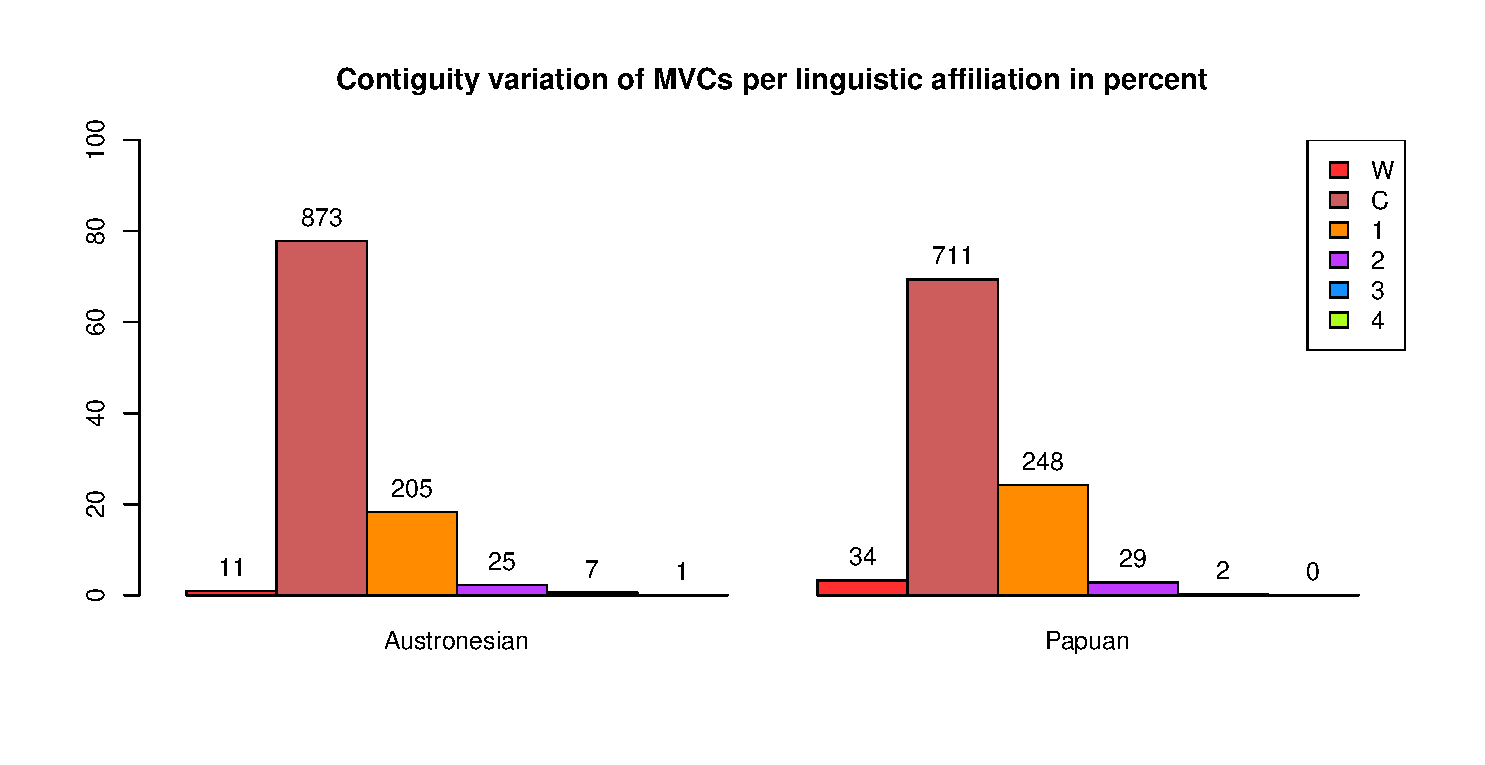
\includegraphics[width=\columnwidth]{figures/Contiguity_Family.eps}
\caption[Contiguity of MVCs by linguistic affiliation]{Contiguity of MVCs by linguistic affiliation in percent. W = Within word, C = Contiguous verbs 1 = One non-verbal constituent intervening, 2 = Two non-verbal constituents intervening, 3 = Three non-verbal constituents intervening, 4 = Four non-verbal constituents intervening. Numbers on top of the bars refer to the number of observations in the sample.}\label{fig:adj-family}
\end{figure}
\begin{figure}
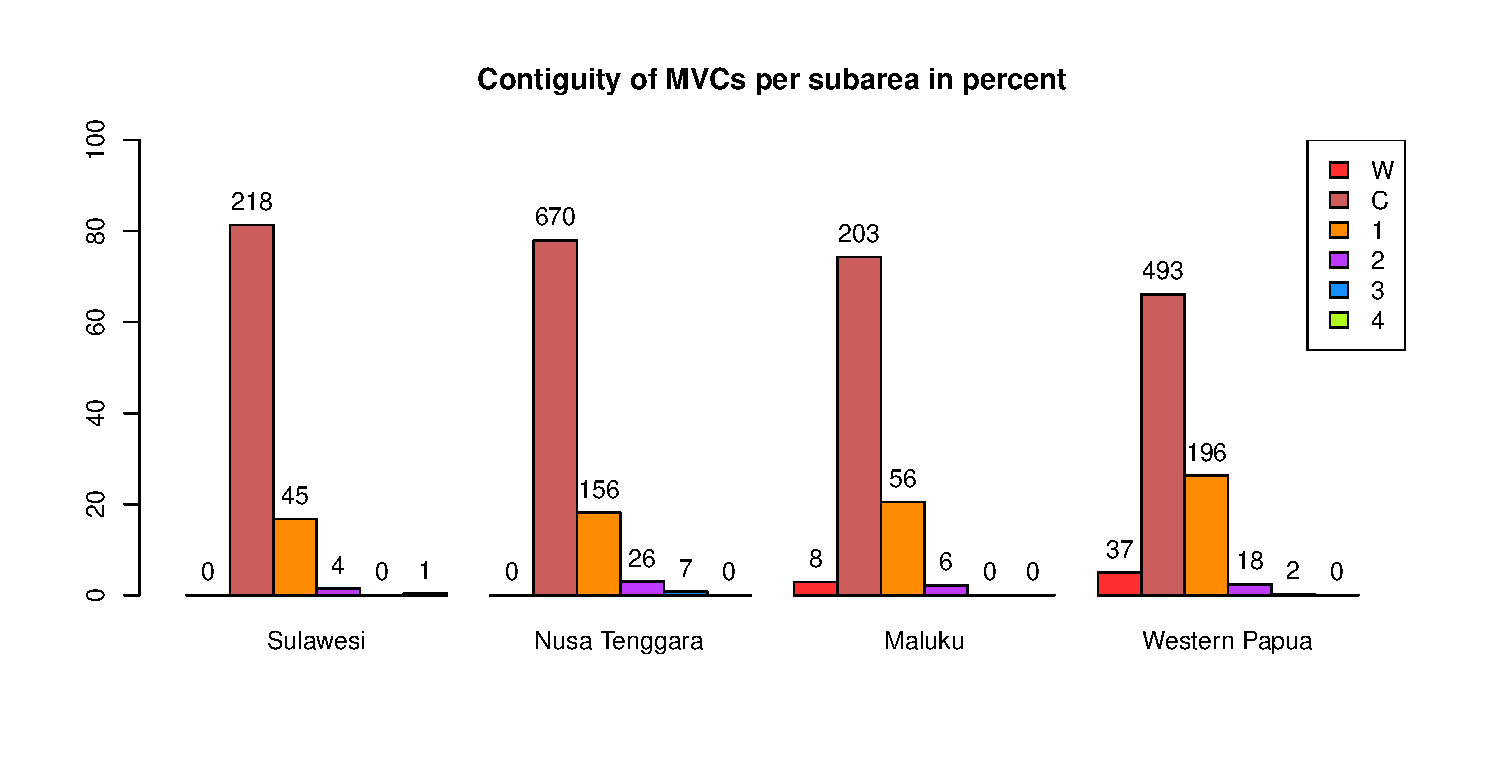
\includegraphics[width=\columnwidth]{figures/Contiguity_Group.eps}
\caption[Contiguity of MVCs by subarea]{Contiguity of MVCs by subarea in percent. W = Within word, C = Contiguous verbs 1 = One non-verbal constituent intervening, 2 = Two non-verbal constituents intervening, 3 = Three non-verbal constituents intervening, 4 = Four non-verbal constituents intervening. Numbers on top of the bars refer to the number of observations in the sample.}\label{fig:adj-group}
\end{figure}

\begin{table}
\begin{tabular}{lrrrrrr}
  \lsptoprule
 & \multicolumn{1}{c}{W} & \multicolumn{1}{c}{C} & \multicolumn{1}{c}{1} & \multicolumn{1}{c}{2} & \multicolumn{1}{c}{3} & \multicolumn{1}{c}{4} \tabularnewline 
  \midrule
  Muna &   0 &  34 &  13 &   2 &   0 &   1 \tabularnewline 
  Pendau &   0 &  45 &   6 &   0 &   0 &   0 \tabularnewline 
  Tajio &   0 &  24 &   8 &   0 &   0 &   0 \tabularnewline 
  Tolaki &   0 &  54 &  9 &   2 &   0 &   0 \tabularnewline 
  Tukang Besi &   0 &  61 &   9 &   0 &   0 &   0 \tabularnewline \midrule
  Abui &   0 &  93 &  15 &   1 &   0 &   0 \tabularnewline 
  Alorese &   0 &  33 &  13 &   1 &   0 &   0 \tabularnewline 
  Bunaq &   0 &  70 &  17 &   0 &   0 &   0 \tabularnewline 
  Kaera &   0 &  13 &  9 &   2 &   0 &   0 \tabularnewline 
  Kambera &   0 &  41 &   3 &   0 &   0 &   0 \tabularnewline 
  Klon &   0 &  76 &  21 &   3 &   0 &   0 \tabularnewline 
  Makalero &   0 &  67 &  8 &   1 &   0 &   0 \tabularnewline 
  Teiwa &   0 &  63 &  19 &   2 &  1 &   0 \tabularnewline 
  Tetun &   0 &  57 &  16 &   0 &   0 &   0 \tabularnewline 
  Waimaqa &   0 & 126 &  29 &  15 &   6 &   0 \tabularnewline 
  Western Pantar &   0 &  31 &   6 &   1 &   0 &   0 \tabularnewline \midrule
  Buru & 8 & 51 & 9 & 0 & 0 & 0 \tabularnewline
  Selaru &   0 &  17 &  7 &  1 &   0 &   0 \tabularnewline 
  Taba &   0 &  34 &  10 &   0 &   0 &   0 \tabularnewline 
  Tidore & 0 & 66 & 22 & 4 & 0 & 0 \tabularnewline
  Tobelo &   0 &  35 &  8 &   1 &   0 &   0 \tabularnewline 
\midrule
  Abun &   0 &  19 &  14 &   0 &   0 &   0 \tabularnewline 
  Biak &   0 &  51 &  15 &   1 &   0 &   0 \tabularnewline 
  Dusner &   0 &  28 &  21 &   0 &   0 &   0 \tabularnewline 
  Hatam &   0 &  25 &  22 &   2 &   0 &   0 \tabularnewline 
  Inanwatan &  20 &  5 &   1 &   2 &   0 &   0 \tabularnewline
  Maybrat &   0 &  55 &  23 &   0 &   0 &   0 \tabularnewline 
  Mor &   0 &  62 &  6 &   2 &   1 &   0 \tabularnewline 
  Moskona &   0 &  41 &  35 &   3 &   0 &   0 \tabularnewline 
  Mpur &   1 &  39 &  19 &   3 &   0 &   0 \tabularnewline 
  Sougb &  13 &   13 &  9 &   4 &   1 &   0 \tabularnewline 
  Wooi &   3 & 155 &  31 &   1 &   0 &   0\tabularnewline 
   \lspbottomrule
\end{tabular}
\caption[Contiguity variation by language]{Contiguity variation by language. W = Within word, C = Contiguous verbs 1 = One non-verbal constituent intervening, 2 = Two non-verbal constituents intervening, 3 = Three non-verbal constituents intervening, 4 = Four non-verbal constituents intervening.}
\label{table:Contiguity_per_lang}
\end{table}

When we turn to contiguity variation by language (cf. \tabref{table:Contiguity_per_lang}) we see that the distribution is again quite even across the EI languages. What seems surprising is that there is not a single language that seems to use just one of the patterns for all its MVCs: All languages have MVCs with contiguous verbs, and others with non-contiguous verbs. Certain constructions may be predisposed towards specific contiguity patterns (e.g., motion constructions might tend towards ``C" because V$_1$ typically hosts an intransitive verb so that no direct object may go between it and the following verb). Alternatively, certain constructions/ languages may not impose specific restrictions, so that speakers are free to insert non-verbal constituents into any MVC (for instance, adverbials; as long as limits of information-load are not transgressed). 

A closer inspection of the data seems to suggest that both cases in fact contribute to the general pattern. In some languages, certain constructions indeed remain stable, in that a constructional template seems to receive a fixed order of constituents. This is particularily clear in instances of MVCs within a single phonological unit. For instance, in Inanwatan, motion complex constructions involving one motion event that is dissected into two or more verbal event descriptors consistently appear in ``W" construals, as illustrated in (\ref{inanwatan004}) below. The first verb, \textit{mogó} `carry', remains uninflected and attaches to the second verb or verbal complex (like \textit{de-wo} in the example), which is inflected for person and syntactic function (prefix), as well as for tense, number and gender (suffix).

\ea \label{inanwatan004}
\langinfo{Inanwatan}{Papuan, SBH}{\citealt[44]{devries2004}}\\
\gll mái-wo wó-uwu-i ewáiwa, ao nésar áwuga-era-era-ro tétewo mogó-we-de-wo-i \\
here-to 3\textsc{sbj}-sit-\textsc{pst}.\textsc{sg}.\textsc{m} and his smithy iron-piece-piece-\textsc{pl} all carry-3\textsc{sbj}-go.across-come-\textsc{pst}.\textsc{sg}.\textsc{m} \\
\glft `Here he settled, and he brought across pieces of iron for his smithy.'\\ 
\z

Verb contiguity is thus in many cases directly influenced by properties more general to the given language: as would be expected in verb-final languages like Inanwatan, the object of the transport verb \textit{mogo} precedes the verbal complex. Similar constructions in verb-second languages confirm this: the object of the transport verb in V$_1$ appears postverbally and thus before V$_2$, typically leading to a ``1" pattern if the theme argument of the transport process is expressed. (\ref{pendau016}) is an example from Pendau:

\ea  \label{pendau016}
\langinfo{Pendau}{Austronesian, WMP}{\citealt[345]{Quick2007}}\\
\glll io nongkomung tuainyo uo manyau rigii nudagat \\
io N-pong-'omung tuai=nyo 'uo ma-nyau ri=gii nu=dagat \\
3\textsc{sg}.\textsc{abs} \textsc{rls}-\textsc{sf}-carry y.sibling=3\textsc{sg}.\textsc{gen} yonder \textsc{ug}:\textsc{irr}-go.down \textsc{loc}=edge \textsc{cn}:\textsc{gen}=ocean \\
\glft `She carried her baby sister down to the edge of the ocean.'\\
\z

Certain constructions may on the other hand allow for variation with regard to interverbal constituents. Motion-to-action constructions in Waima'a, for instance, are commonly construed with the ``C" pattern (as in (\ref{waimaqa003}) below). However, up to three constituents may occur between the verbs, as in example (\ref{waimaqa004}), where an adverbial (\textit{nan}), a goal NP (\textit{basara}) and a proform (\textit{wuo-ruo}) are placed before V$_2$ which saturates the action slot of the motion-to-action template.\footnote{Note that in Waima'a MVCs may occur without an overt subject associated with V$_1$. In such cases, the overt subject may appear before V$_2$. This is very likely related to information-structural issues. The phenomenon bears a resemblance to tail-head linkage systems in that old information from the previous IP is often repeated as the first part of the ongoing IP. Overt subject assignment probably indicates new information in such construals. I did not filter out such MVCs, but a thorough analysis might prove that these instances are in fact better treated as some kind of information-structural device repeating known information in a condensed form. This issue is indeed vital for MVC analysis, and my hypothesis is that \textsc{stage-relating construction}s of at least some types are brought to life by such a device. I will explore this question briefly as an outlook to further research in Chapter \ref{ch:discussion}.}

\ea \label{waimaqa003}
\langinfo{Waima'a}{Austronesian, CMP}{dom2\_kaben 61}\\
\gll ne mai sani loli se ehe \\
3\textsc{sg} come sing expression one say \\
\glft `Someone comes speaking in `loli' language saying...'\\ 
\z

\ea \label{waimaqa004}
\langinfo{Waima'a}{Austronesian, CMP}{dom2\_kaben 22--3}\\
\glll kas nan basara wuo-ruo hita ini \\ 
laka\_isi nani basara wuo-ruo hita ini \\
go\_\textsc{prep?} perhaps market \textsc{clf}-two find \textsc{recp} \\
\glft `Going to the market the two would meet.'\\ 
\z

In the following sections, I will provide some more examples of contiguous and non-contiguous constructions. 

\subsubsection{Contiguous constructions}

Contiguous constructions \textit{sensu lato} comprise both within-word contiguity and verbal adjacency (the ``C" pattern). As the latter is the unmarked choice for MVCs in Eastern Indonesia, I will here turn to some more examples of the ``W" type. Within-word contiguity only appears in a small subset of languages of Western Papua and the Moluccas. While Inanwatan shows a variety of different constructions, all construed as ``W", the Sougb cases are mostly confined to motion MVCs. Only three verbs are found in V$_1$ position: \textit{ed(a)/d} `go', \textit{en} `come', and \textit{ougb} `run'. V$_2$ may host a variety of action and motion verbs, deriving motion-to-action MVCs or motion complex MVCs. Example (\ref{sougb001}) is a typical case of the motion-to-action scenario. (\ref{sougb002}) gives a motion complex with a manner of motion verb in front and a path-specifying directed motion verb in second position (note that the whole MVC is a subordinated relative clause derived by the use of a nominaliser).

\ea \label{sougb001}
\langinfo{Sougb}{Papuan, EBH}{\citealt[214]{reesink2002grammar}}\\
\gll Ban b-in naugb b-id-eya se ab-ires habi. \\
you 2\textsc{sg}-come for 2\textsc{sg}-go-see with 2\textsc{sg}-eye then \\
\glft `You come to go see (him) with your own eyes first.'\\ 
\z

\ea \label{sougb002}
\langinfo{Sougb}{Papuan, EBH}{\citealt[200]{reesink2002grammar}}\\
\gll Godeh hom g-ougb-da dau m-ena. \\
child one \textsc{nm}-run-go from 3\textsc{sg}-father \\
\glft `A son who ran away from his father.'\\ 
\z

Another use of the within-word pattern in Sougb MVCs is required by the loanword verbaliser \textit{(e)be} that is glossed as `do'. In order to integrate loanverbs and use them as verbs, \textit{(e)be} has to be attached carrying a subject indexing prefix, as shown by example (\ref{sougb003}) (\textit{menghadap} is a loanverb from Indonesian, fully integrated - even with the actor voice prefix \textit{meN-} - into Sougb).

\ea \label{sougb003}
\langinfo{Sougb}{Papuan, EBH}{\citealt[217]{reesink2002grammar}}\\
\gll Tau la-(e)be-menghadap-im. \\
or 2\textsc{du}-do-oppose-\textsc{recp} \\
\glft `Or the two of them were opposite to each other.'\\
\z

Further traces of within-word MVCs can be found in lexicalised verb compounds in Sougb (some items are listed in \citealt[216]{reesink2002grammar}). Complex word formation with more than one verbal morpheme is also occasionally found in other languages of the area, most notably in Abui for which \citet{kratochvil2007grammar} discusses quite complex formation patterns. As many of these compound verbs seem to have lost a great deal of their internal semantics, I generally refrained from recording them as MVCs proper, though more in-depth analyses of fixed complex verbs might still find that the semantic patterns from the EI sample are in fact of the same (or at least of a similar) kind.

In Wooi, three cases of within-word MVCs have been recorded, two of them involving the generic verb \textit{ong} in the sense of \textit{ong} x = follow x = doing also x. \textit{Ong} always comes first and forms what I call a sequitive construction. In most instances, both verbs behave like fully independent verbs, yet in the following two cases a sandhi effect appears between the verbs. This suggests that they are more fully integrated here. In (\ref{wooi003}) the fricative /v/ is changed to the homorganic voiced stop [b] which in turn causes the morpheme-final nasal /n/ (in its word-final allophone [ng]) to assimilate to [m]. Example (\ref{wooi004}) illustrates another sandhi between two morphemes: here, a combination of two morphemes causes the segment /s/ to appear in its word-internal form [s] (instead of the allophone [h] which appears in word-initial position\footnote{The spelling [hn] in Wooi reflects a nasalisation of the glottal fricative, appearing before high vowels /u/ and /i/.}). The change of [h] to [s] in \textit{cosua} strongly suggests that both morphemes form a tight phonological unit, and therefore are best treated as a ``W" MVC.

\ea \label{wooi003}
\langinfo{Wooi}{Austronesian, SHWNG}{midwife\_traditional\_medicine 21--2}\\
\glll tangko na yampa konta varo combemengerti \\
ta-ko na yampa konta varomi ti-ong-ve-mengerti \\
1\textsc{pl}.\textsc{in}-take \textsc{abl} \textsc{med} again in.order.to 3\textsc{sg}-follow-\textsc{vblz}-understand \\
\glft `We have to take (knowledge) from it as well, so that she also understands.'\\ 
\z

\ea \label{wooi004}
\langinfo{Wooi}{Austronesian, SHWNG}{zaman\_Belanda 118}\\
\glll bertindak kio cosua \\
bertindak kio ti-ong-hnua \\
operate until 3\textsc{sg}-follow-enter \\
\glft `He (the Dutch) ruled until he (the Japanese) also came in.'\\ 
\z

What the Wooi cases demonstrate is that there may be both languages that adopt a ``W" pattern by way of grammaticalisation of a specific construction, and other languages in which the exact formation of some MVC may be subject to a certain amount of free inter-speaker variation. Both Wooi speakers that produced the utterances in (\ref{wooi003}) and (\ref{wooi004}) were old speakers, 84 and 78 years old respectively. The variation evident in the examples above may therefore in fact reflect inter-generational differences in MVC formation and use, rather than a constructional property.

\subsubsection{Non-contiguous constructions}

The verbs of non-contiguous MVCs are separated by one or more constituents. One constituent is the most frequent pattern, but up to four constituents have been recorded before the second verb of the construction. Extreme cases tend to belong to MVC categories that are typically not analysed as SVCs, for instance because the (subject) referents are not shared by the verbs (\textsc{free juxtaposition}). The only case of ``4" in the sample is a good example.

\ea \label{Muna047}
\langinfo{Muna}{Austronesian, WMP}{\citealt[343]{vandenberg1989}}\\
\gll ka-rimba-no no-horo katogha ka-rimba-no dua dahu no-lumpa \\
\textsc{nm}-fast-\textsc{poss} 3\textsc{sg}.\textsc{rls}-fly crow \textsc{nm}-fast-\textsc{poss} also dog 3\textsc{sg}.\textsc{rls}-run \\
\glft `The faster the crow flew, the faster the dog ran.' (lit. `its fastness, the crow flew, its fastness also the dog ran')\\ 
\z

In example (\ref{Muna047}) from Muna, the verbs are separated from one another by four constituents: the postponed subject \textit{katogha}, a \textit{ka}-nominalisation of the verb \textit{rimba}, an adverb \textit{dua}, and the second subject \textit{dahu}. This is an example that is taken from one of the appended texts. While van den Berg did make use of punctuation throughout the text, marking (potential) points of prosodic segmentation, the case in (\ref{Muna047}) could probably also be uttered in two IPs. Furthermore, only the second part of the utterance is modified by the adverb. This seems to point at a biclausal construal rather than a MVC. At the same time, the interpretation is clearly that of a construction with fixed semantics (the more X, the more Y). Cases like this one are hard to interpret and should at this analytical stage at best be understood as peripheral examples of MVCs.

More typical cases of discontinuous MVCs are illustrated by the following examples. We see that a range of different elements can fill the position between the verb constituents. Some, as the goal argument \textit{turu uling} in example (\ref{alorese_bed}) from Alorese, are directly licensed by the preceding verb. Other elements are adjuncts (as \textit{hanyen} and \textit{bu} in example (\ref{hatam_walk}) from Hatam), or pertain to partial modification of one of the constructional stages (as with the aspectual marker \textit{lo} that aligns with the right edge of the motion \textsc{stage} in example (\ref{waimaqa_come})).

\ea \label{alorese_bed}
\langinfo{Alorese}{Austronesian, CMP}{\citealt[130]{klamer2011alorese}}\\
\gll mareng lele neka, fe gere turu uling hiki turu \\
night long already they go.up sleep place see sleep \\
\glft `In the middle of the night, they get into bed to sleep.'\\ 
\z

\ea \label{hatam_walk}
\langinfo{Hatam}{Papuan, Hatam-Mansim}{\citealt[97]{reesink1999grammar}}\\
\gll nok lene ni-mbut hanyen bu ni-kwei ei igbei \\
like then 1\textsc{ex}-walk anew again 1\textsc{ex}-come \textsc{loc} house \\
\glft `So then we walked around again, came home ...'\\ 
\z

\ea \label{waimaqa_come}
\langinfo{Waima'a}{Austronesian, CMP}{pear\_Santina 203}\\
\gll mai lo bati la \\
come \textsc{asp} divide \textsc{loc} \\
\glft `(One of them came running), he came to divide (it) up.'\\ 
\z

\section{Summary}

Summarising the findings from this chapter, I have introduced and discussed three formal parameters that are retrievable from published data sources: (i) argument sharing, (ii) headedness, and (iii) contiguity. A quantitative assessment revealed that the EI languages in fact differ very little across the preferred features. For neither of the three parameters could a strong influence of genealogical affiliation be found. In headedness variation, however, there is a tendency for the Papuan languages to make less use of the head-first pattern than the Austronesian languages. An investigation of the geographical distribution across the four subareas did also not yield clear differences among the groups.

What can be gathered from the sample is that prototypical MVCs in the EI area have shared subject arguments (``S"), that both verbs bear the same amount of inflection (``B"), and that they occur right next to each other (``C") without intervening constituents such as direct object arguments or adjuncts. This is in line with van Staden and Reesink's finding that ``independent serialisation is by far the most commonly found type" \citep[48]{vanstaden2008serial}. This holds all the more if we include the isolating languages Alorese, Waima'a, and Buru into the picture. These languages do not possess any other strategy than to construe MVCs without verbal morphology (and thus appear to be symmetrical in terms of headedness as well). Another finding can also be supported: that co-dependent serialisation (involving argument switch of the ``D" type) is very common (especially for change of state, as we shall see in section \sectref{sec:causation}). In \sectref{sec:argumentstructure}, the numbers not only showed a moderate degree of ``D" type argument sharing patterns, but also that virtually every EI language in the sample makes use of them. Switch-subject constructions can therefore be regarded a general trait across all of Wallacea (as the use of MVCs in general).

What the data have shown is that variation in the morphosyntactic make-up of MVCs is a poor predictor of areal tendencies or genealogical descendance of the languages. It seems, therefore, that van Staden \& Reesink's conclusion that ``serialisation on the whole is more characteristic of the Papuan languages than of the Austronesian languages" \citep[50]{vanstaden2008serial} is not borne out by evidence from the present sample. From a formal perspective, it appears that variation in formal encoding of MVCs is characteristic of all languages. In the next chapter, I will shift my focus to semantic properties of MVCs, arguing for a distinction into three basic techniques of MVC formation: feature \textsc{merging}, \textsc{modification}, and \textsc{staging}.
